\documentclass[10pt]{article}
% Combined PDF of the PNAS paper (wellbeing_pnas.tex) and its SI Appendix (wellbeing_pnas_si.tex), with clickable links
% between the two: references to SI tables in the main text link to them, and each SI table or figure links back to
% the place citing it ("Back to Results", "Back to Section S2"...). Both files are included as is (package docmute).
% Compile from papers/:  latexmk -pdf -outdir=build wellbeing_pnas_combined.tex
\usepackage[T1]{fontenc}
\usepackage[utf8]{inputenc}
\usepackage{mathpazo}
\usepackage[margin=2cm]{geometry}
\usepackage[numbers,round,sort&compress]{natbib}
\usepackage{graphicx, booktabs, adjustbox, amsmath, amssymb, xcolor, caption, lineno, makecell, threeparttable}
\captionsetup{font=small, labelfont=bf}
\usepackage[colorlinks=true, urlcolor=purple, linkcolor=blue, citecolor=violet]{hyperref}
\usepackage{xspace}
\xspaceaddexceptions{]\%}
\newcommand{\corGallupWHR}{0.993\xspace}
\newcommand{\corGallupWHRoldMapping}{0.89\xspace}
\newcommand{\nGallupCountryYears}{2351\xspace}
\newcommand{\nGallupCountries}{168\xspace}
\newcommand{\nWVSCountryYears}{304\xspace}
\newcommand{\nWVSCountries}{108\xspace}
\newcommand{\nWVSRespondents}{439531\xspace}
\newcommand{\nFabre}{11000\xspace}
\newcommand{\nFabreCountries}{10\xspace}
\newcommand{\bestIncome}{Cluster k=7 nominal\xspace}
\newcommand{\shareRegionBetterWVS}{86\xspace}
\newcommand{\shareRegionBetterWVSbest}{79\xspace}
\newcommand{\nSpecsWVS}{952\xspace}
\newcommand{\meanShareIncomeBest}{28\xspace}
\newcommand{\meanRtwoIncomeBest}{19\xspace}
\newcommand{\meanRtwoIncomePPP}{12\xspace}
\newcommand{\meanRtwoRegion}{37\xspace}
\newcommand{\RtwoSatisfiedMeanPPP}{20\xspace}
\newcommand{\RtwoHappinessMeanPPP}{4\xspace}
\newcommand{\RtwoVeryHappyPPP}{0\xspace}
\newcommand{\shareRegionBetterGallup}{35\xspace}
\newcommand{\shareIncomeGallupMean}{60\xspace}
\newcommand{\RtwoGallupMeanPPP}{61\xspace}
\newcommand{\RtwoGallupRegion}{48\xspace}
\newcommand{\RtwoWHRPPP}{63\xspace}
\newcommand{\RtwoWHRRegion}{55\xspace}
\newcommand{\shareRegionBetterNoLatamEE}{27\xspace}
\newcommand{\shareIncomeNoLatamEE}{34\xspace}
\newcommand{\shareRegionBetterContinents}{54\xspace}
\newcommand{\shareRegionBetterWB}{64\xspace}
\newcommand{\cvIncomeSatisfiedMean}{0.18\xspace}
\newcommand{\cvRegionSatisfiedMean}{0.44\xspace}
\newcommand{\cvIncomeGallupMean}{0.60\xspace}
\newcommand{\cvRegionGallupMean}{0.45\xspace}
\newcommand{\shareCvRegionBetterWVS}{100\xspace}
\newcommand{\corHappySatisfied}{0.72\xspace}
\newcommand{\corHappinessSatisfactionMean}{0.76\xspace}
\newcommand{\corVeryHappySatisfiedMean}{0.63\xspace}
\newcommand{\slopeVeryHappy}{0.005\xspace}
\newcommand{\pVeryHappy}{0.85\xspace}
\newcommand{\happiestFirst}{Switzerland\xspace}
\newcommand{\happiestFirstN}{10\xspace}
\newcommand{\happiestSecond}{Mexico\xspace}
\newcommand{\happiestSecondN}{9\xspace}
\newcommand{\happiestThird}{Kyrgyzstan\xspace}
\newcommand{\happiestThirdN}{6\xspace}
\newcommand{\happiestRegionWestern}{24\xspace}
\newcommand{\happiestRegionLatinAmerica}{19\xspace}
\newcommand{\happiestRegionAsia}{16\xspace}
\newcommand{\happiestRegionAfrica}{5\xspace}
\newcommand{\nHappiestCells}{64\xspace}
\newcommand{\treeRegionFirst}{8\xspace}
\newcommand{\withinRtwoSatisfiedMean}{0.22\xspace}
\newcommand{\withinSlopeSatisfiedMean}{1.68\xspace}
\newcommand{\crossSlopeSatisfiedMean}{1.09\xspace}
\newcommand{\withinSlopeVeryHappy}{0.18\xspace}
\newcommand{\pWithinVeryHappy}{0.004\xspace}
\newcommand{\nWithin}{272\xspace}
\newcommand{\RtwoFreedomSatisfaction}{63\xspace}
\newcommand{\shapleyFreedom}{40\xspace}
\newcommand{\shapleyFreedomRegion}{26\xspace}
\newcommand{\shapleyFreedomIncome}{9\xspace}
\newcommand{\RtwoTolerance}{21\xspace}
\newcommand{\RtwoGod}{0\xspace}
\newcommand{\RtwoGrowth}{2\xspace}
\newcommand{\nonresponseSatisfactionWVS}{1.5\xspace}
\newcommand{\nonresponseHappinessWVS}{1.7\xspace}
\newcommand{\corNonresponseGDP}{-0.08\xspace}
\newcommand{\effectLadder}{-0.45\xspace}
\newcommand{\seLadder}{0.05\xspace}
\newcommand{\effectScale}{0.14\xspace}
\newcommand{\seScale}{0.05\xspace}
\newcommand{\effectLadderZeroTen}{-0.46\xspace}
\newcommand{\effectScaleZeroTen}{-0.26\xspace}
\newcommand{\effectLadderSatisfied}{-9\xspace}
\newcommand{\interactionLadderIncome}{-0.004\xspace}
\newcommand{\pInteractionLadderIncome}{0.92\xspace}
\newcommand{\gradientIncomeSatisfaction}{0.69\xspace}
\newcommand{\pHeterogeneityWording}{0.000\xspace}
\newcommand{\chiHeterogeneityWording}{93.4\xspace}
\newcommand{\wordingCHE}{-0.34\xspace}
\newcommand{\wordingDEU}{-0.53\xspace}
\newcommand{\wordingESP}{-1.12\xspace}
\newcommand{\wordingFRA}{-0.50\xspace}
\newcommand{\wordingGBR}{-0.63\xspace}
\newcommand{\wordingITA}{-0.55\xspace}
\newcommand{\wordingJPN}{0.36\xspace}
\newcommand{\wordingPOL}{-0.55\xspace}
\newcommand{\wordingSAU}{-0.79\xspace}
\newcommand{\wordingUSA}{-0.63\xspace}
\newcommand{\wordingMin}{-1.12\xspace}
\newcommand{\wordingMax}{0.36\xspace}
\newcommand{\decompMeanGap}{-0.39\xspace}
\newcommand{\decompMeanQuestion}{-0.71\xspace}
\newcommand{\decompMeanResidual}{0.32\xspace}
\newcommand{\decompShareLevelQuestion}{1.83\xspace}
\newcommand{\decompVarShareQuestion}{-0.20\xspace}
\newcommand{\decompVarShareResidual}{1.20\xspace}
\newcommand{\decompMeanAbsGap}{0.43\xspace}
\newcommand{\decompMeanAbsResidual}{0.64\xspace}
\newcommand{\decompRmsePredictionGallup}{0.73\xspace}
\newcommand{\decompRmseNaive}{0.42\xspace}
\newcommand{\decompMeanGapSat}{-0.05\xspace}
\newcommand{\decompMeanQuestionSat}{-0.11\xspace}
\newcommand{\decompVarShareQuestionSat}{-0.11\xspace}
\newcommand{\decompSdGap}{0.44\xspace}
\newcommand{\decompSdQuestion}{0.45\xspace}
\newcommand{\decompSdResidual}{0.69\xspace}
\newcommand{\decompCorGapQuestion}{-0.20\xspace}
\newcommand{\decompLowMeanGap}{-0.44\xspace}
\newcommand{\decompHighMeanGap}{-0.34\xspace}
\newcommand{\decompLowMeanQuestion}{-0.85\xspace}
\newcommand{\decompHighMeanQuestion}{-0.56\xspace}
\newcommand{\decompLowMeanResidual}{0.17\xspace}
\newcommand{\decompHighMeanResidual}{0.46\xspace}
\newcommand{\decompLowVarShareQuestion}{-0.52\xspace}
\newcommand{\decompHighVarShareQuestion}{0.15\xspace}
\newcommand{\decompLowShareLevelQuestion}{1.42\xspace}
\newcommand{\decompHighShareLevelQuestion}{2.27\xspace}
\newcommand{\decompLowCorGapQuestion}{-0.47\xspace}
\newcommand{\decompHighCorGapQuestion}{0.14\xspace}
\newcommand{\nDecompCountries}{10\xspace}
\newcommand{\nSameYear}{7\xspace}
\newcommand{\nRecent}{4\xspace}
\newcommand{\varShareQuestionSameYear}{-0.27\xspace}
\newcommand{\varShareQuestionRecent}{-0.81\xspace}
\newcommand{\shareLevelQuestionSameYear}{1.60\xspace}
\newcommand{\shareLevelQuestionRecent}{1.19\xspace}
\newcommand{\meanSampleEffectGallup}{0.75\xspace}
\newcommand{\corFabreWHR}{0.75\xspace}
\newcommand{\minSampleEffectGallup}{0.16\xspace}
\newcommand{\maxSampleEffectGallup}{1.24\xspace}
\newcommand{\meanSampleEffectWVS}{0.54\xspace}
\newcommand{\meanFabreGallupZero}{5.93\xspace}
\newcommand{\meanFabreWVSOne}{6.64\xspace}
\newcommand{\sampleEffectUSWVS}{0.49\xspace}
\newcommand{\nCommon}{149\xspace}
\newcommand{\nCommonCountries}{83\xspace}
\newcommand{\RtwoCommonGallup}{0.49\xspace}
\newcommand{\RtwoCommonWVS}{0.11\xspace}
\newcommand{\slopeCommonGallup}{1.76\xspace}
\newcommand{\slopeCommonWVS}{0.77\xspace}
\newcommand{\slopeGapGDP}{1.07\xspace}
\newcommand{\seSlopeGapGDP}{0.16\xspace}
\newcommand{\RtwoGapGDP}{0.31\xspace}
\newcommand{\slopeQuestionGDP}{0.30\xspace}
\newcommand{\seSlopeQuestionGDP}{1.75\xspace}
\newcommand{\RtwoAdjustedWVS}{0.20\xspace}
\newcommand{\shareIncomeCommonGallup}{51\xspace}
\newcommand{\shareIncomeCommonWVS}{15\xspace}

\providecommand{\newsurvey}{Fabre (2025)\xspace}
\newcommand{\Rsq}{\ensuremath{R^2}\xspace}
\bibliographystyle{unsrtnat}
\usepackage{docmute}

% Main text: references to SI tables are links; the first citation of each table is the target of its back-link
\newcommand{\SIref}[3]{\ifcsname SIback@#1\endcsname\else\expandafter\gdef\csname SIback@#1\endcsname{#3}\phantomsection\label{back:#1}\fi\ref{#1}}
% SI Appendix: back to the main text if the table is cited there, otherwise back to the SI section citing it
\newcommand{\backlink}[2]{\ifcsname SIback@#1\endcsname\hfill\hyperref[back:#1]{(Back to \csname SIback@#1\endcsname, main text)}%
  \else\if\relax\detokenize{#2}\relax\else\hfill\hyperref[#2]{(Back to Section~\ref*{#2})}\fi\fi}

\title{Whether richer countries are happier depends on the survey}
\author{Adrien Fabre\\ \small CNRS, CIRED, Paris, France. \href{mailto:adrien.fabre@cnrs.fr}{adrien.fabre@cnrs.fr}. ORCID: \href{https://orcid.org/0000-0001-5245-7772}{0000-0001-5245-7772}}
\date{}

\begin{document}
\documentclass[10pt]{article}
% PNAS version (Research Report, Social Sciences / Economic Sciences; secondary: Psychological and Cognitive Sciences).
% PNAS has a format-neutral policy for initial submissions: this file follows the PNAS structure (abstract <= 250 words,
% significance statement <= 120 words, untitled introduction, Results, Discussion, Materials and Methods, numbered references,
% ~6 pages / ~4,000 words, 3 display items); after acceptance, transfer the text into the official PNAS LaTeX template (Overleaf).
% Submission track: Direct Submission.
% Supporting information: wellbeing_pnas_si.tex (SI Appendix). Compile from papers/, twice each:
%   latexmk -pdf -outdir=build wellbeing_pnas.tex ; latexmk -pdf -outdir=build wellbeing_pnas_si.tex
% References to the SI Appendix (Table S1, S3...) are written as plain numbers so that this file compiles on its own:
% update them if the order of tables in wellbeing_pnas_si.tex changes.
\usepackage[T1]{fontenc}
\usepackage[utf8]{inputenc}
\usepackage{mathpazo}
\usepackage[margin=2cm]{geometry}
\usepackage[numbers,round,sort&compress]{natbib}
\usepackage{graphicx, booktabs, adjustbox, amsmath, amssymb, xcolor, caption, lineno}
\captionsetup{font=small, labelfont=bf}
\usepackage[colorlinks=true, urlcolor=purple, linkcolor=blue, citecolor=violet]{hyperref}
\usepackage{xspace}
\xspaceaddexceptions{]\%}
\newcommand{\corGallupWHR}{0.993\xspace}
\newcommand{\corGallupWHRoldMapping}{0.89\xspace}
\newcommand{\nGallupCountryYears}{2351\xspace}
\newcommand{\nGallupCountries}{168\xspace}
\newcommand{\nWVSCountryYears}{304\xspace}
\newcommand{\nWVSCountries}{108\xspace}
\newcommand{\nWVSRespondents}{439531\xspace}
\newcommand{\nFabre}{11000\xspace}
\newcommand{\nFabreCountries}{10\xspace}
\newcommand{\bestIncome}{Cluster k=7 nominal\xspace}
\newcommand{\shareRegionBetterWVS}{86\xspace}
\newcommand{\shareRegionBetterWVSbest}{79\xspace}
\newcommand{\nSpecsWVS}{952\xspace}
\newcommand{\meanShareIncomeBest}{28\xspace}
\newcommand{\meanRtwoIncomeBest}{19\xspace}
\newcommand{\meanRtwoIncomePPP}{12\xspace}
\newcommand{\meanRtwoRegion}{37\xspace}
\newcommand{\RtwoSatisfiedMeanPPP}{20\xspace}
\newcommand{\RtwoHappinessMeanPPP}{4\xspace}
\newcommand{\RtwoVeryHappyPPP}{0\xspace}
\newcommand{\shareRegionBetterGallup}{35\xspace}
\newcommand{\shareIncomeGallupMean}{60\xspace}
\newcommand{\RtwoGallupMeanPPP}{61\xspace}
\newcommand{\RtwoGallupRegion}{48\xspace}
\newcommand{\RtwoWHRPPP}{63\xspace}
\newcommand{\RtwoWHRRegion}{55\xspace}
\newcommand{\shareRegionBetterNoLatamEE}{27\xspace}
\newcommand{\shareIncomeNoLatamEE}{34\xspace}
\newcommand{\shareRegionBetterContinents}{54\xspace}
\newcommand{\shareRegionBetterWB}{64\xspace}
\newcommand{\cvIncomeSatisfiedMean}{0.18\xspace}
\newcommand{\cvRegionSatisfiedMean}{0.44\xspace}
\newcommand{\cvIncomeGallupMean}{0.60\xspace}
\newcommand{\cvRegionGallupMean}{0.45\xspace}
\newcommand{\shareCvRegionBetterWVS}{100\xspace}
\newcommand{\corHappySatisfied}{0.72\xspace}
\newcommand{\corHappinessSatisfactionMean}{0.76\xspace}
\newcommand{\corVeryHappySatisfiedMean}{0.63\xspace}
\newcommand{\slopeVeryHappy}{0.005\xspace}
\newcommand{\pVeryHappy}{0.85\xspace}
\newcommand{\happiestFirst}{Switzerland\xspace}
\newcommand{\happiestFirstN}{10\xspace}
\newcommand{\happiestSecond}{Mexico\xspace}
\newcommand{\happiestSecondN}{9\xspace}
\newcommand{\happiestThird}{Kyrgyzstan\xspace}
\newcommand{\happiestThirdN}{6\xspace}
\newcommand{\happiestRegionWestern}{24\xspace}
\newcommand{\happiestRegionLatinAmerica}{19\xspace}
\newcommand{\happiestRegionAsia}{16\xspace}
\newcommand{\happiestRegionAfrica}{5\xspace}
\newcommand{\nHappiestCells}{64\xspace}
\newcommand{\treeRegionFirst}{8\xspace}
\newcommand{\withinRtwoSatisfiedMean}{0.22\xspace}
\newcommand{\withinSlopeSatisfiedMean}{1.68\xspace}
\newcommand{\crossSlopeSatisfiedMean}{1.09\xspace}
\newcommand{\withinSlopeVeryHappy}{0.18\xspace}
\newcommand{\pWithinVeryHappy}{0.004\xspace}
\newcommand{\nWithin}{272\xspace}
\newcommand{\RtwoFreedomSatisfaction}{63\xspace}
\newcommand{\shapleyFreedom}{40\xspace}
\newcommand{\shapleyFreedomRegion}{26\xspace}
\newcommand{\shapleyFreedomIncome}{9\xspace}
\newcommand{\RtwoTolerance}{21\xspace}
\newcommand{\RtwoGod}{0\xspace}
\newcommand{\RtwoGrowth}{2\xspace}
\newcommand{\nonresponseSatisfactionWVS}{1.5\xspace}
\newcommand{\nonresponseHappinessWVS}{1.7\xspace}
\newcommand{\corNonresponseGDP}{-0.08\xspace}
\newcommand{\effectLadder}{-0.45\xspace}
\newcommand{\seLadder}{0.05\xspace}
\newcommand{\effectScale}{0.14\xspace}
\newcommand{\seScale}{0.05\xspace}
\newcommand{\effectLadderZeroTen}{-0.46\xspace}
\newcommand{\effectScaleZeroTen}{-0.26\xspace}
\newcommand{\effectLadderSatisfied}{-9\xspace}
\newcommand{\interactionLadderIncome}{-0.004\xspace}
\newcommand{\pInteractionLadderIncome}{0.92\xspace}
\newcommand{\gradientIncomeSatisfaction}{0.69\xspace}
\newcommand{\pHeterogeneityWording}{0.000\xspace}
\newcommand{\chiHeterogeneityWording}{93.4\xspace}
\newcommand{\wordingCHE}{-0.34\xspace}
\newcommand{\wordingDEU}{-0.53\xspace}
\newcommand{\wordingESP}{-1.12\xspace}
\newcommand{\wordingFRA}{-0.50\xspace}
\newcommand{\wordingGBR}{-0.63\xspace}
\newcommand{\wordingITA}{-0.55\xspace}
\newcommand{\wordingJPN}{0.36\xspace}
\newcommand{\wordingPOL}{-0.55\xspace}
\newcommand{\wordingSAU}{-0.79\xspace}
\newcommand{\wordingUSA}{-0.63\xspace}
\newcommand{\wordingMin}{-1.12\xspace}
\newcommand{\wordingMax}{0.36\xspace}
\newcommand{\decompMeanGap}{-0.39\xspace}
\newcommand{\decompMeanQuestion}{-0.71\xspace}
\newcommand{\decompMeanResidual}{0.32\xspace}
\newcommand{\decompShareLevelQuestion}{1.83\xspace}
\newcommand{\decompVarShareQuestion}{-0.20\xspace}
\newcommand{\decompVarShareResidual}{1.20\xspace}
\newcommand{\decompMeanAbsGap}{0.43\xspace}
\newcommand{\decompMeanAbsResidual}{0.64\xspace}
\newcommand{\decompRmsePredictionGallup}{0.73\xspace}
\newcommand{\decompRmseNaive}{0.42\xspace}
\newcommand{\decompMeanGapSat}{-0.05\xspace}
\newcommand{\decompMeanQuestionSat}{-0.11\xspace}
\newcommand{\decompVarShareQuestionSat}{-0.11\xspace}
\newcommand{\decompSdGap}{0.44\xspace}
\newcommand{\decompSdQuestion}{0.45\xspace}
\newcommand{\decompSdResidual}{0.69\xspace}
\newcommand{\decompCorGapQuestion}{-0.20\xspace}
\newcommand{\decompLowMeanGap}{-0.44\xspace}
\newcommand{\decompHighMeanGap}{-0.34\xspace}
\newcommand{\decompLowMeanQuestion}{-0.85\xspace}
\newcommand{\decompHighMeanQuestion}{-0.56\xspace}
\newcommand{\decompLowMeanResidual}{0.17\xspace}
\newcommand{\decompHighMeanResidual}{0.46\xspace}
\newcommand{\decompLowVarShareQuestion}{-0.52\xspace}
\newcommand{\decompHighVarShareQuestion}{0.15\xspace}
\newcommand{\decompLowShareLevelQuestion}{1.42\xspace}
\newcommand{\decompHighShareLevelQuestion}{2.27\xspace}
\newcommand{\decompLowCorGapQuestion}{-0.47\xspace}
\newcommand{\decompHighCorGapQuestion}{0.14\xspace}
\newcommand{\nDecompCountries}{10\xspace}
\newcommand{\nSameYear}{7\xspace}
\newcommand{\nRecent}{4\xspace}
\newcommand{\varShareQuestionSameYear}{-0.27\xspace}
\newcommand{\varShareQuestionRecent}{-0.81\xspace}
\newcommand{\shareLevelQuestionSameYear}{1.60\xspace}
\newcommand{\shareLevelQuestionRecent}{1.19\xspace}
\newcommand{\meanSampleEffectGallup}{0.75\xspace}
\newcommand{\corFabreWHR}{0.75\xspace}
\newcommand{\minSampleEffectGallup}{0.16\xspace}
\newcommand{\maxSampleEffectGallup}{1.24\xspace}
\newcommand{\meanSampleEffectWVS}{0.54\xspace}
\newcommand{\meanFabreGallupZero}{5.93\xspace}
\newcommand{\meanFabreWVSOne}{6.64\xspace}
\newcommand{\sampleEffectUSWVS}{0.49\xspace}
\newcommand{\nCommon}{149\xspace}
\newcommand{\nCommonCountries}{83\xspace}
\newcommand{\RtwoCommonGallup}{0.49\xspace}
\newcommand{\RtwoCommonWVS}{0.11\xspace}
\newcommand{\slopeCommonGallup}{1.76\xspace}
\newcommand{\slopeCommonWVS}{0.77\xspace}
\newcommand{\slopeGapGDP}{1.07\xspace}
\newcommand{\seSlopeGapGDP}{0.16\xspace}
\newcommand{\RtwoGapGDP}{0.31\xspace}
\newcommand{\slopeQuestionGDP}{0.30\xspace}
\newcommand{\seSlopeQuestionGDP}{1.75\xspace}
\newcommand{\RtwoAdjustedWVS}{0.20\xspace}
\newcommand{\shareIncomeCommonGallup}{51\xspace}
\newcommand{\shareIncomeCommonWVS}{15\xspace}

\bibliographystyle{unsrtnat}
\renewcommand{\thetable}{\arabic{table}}

\title{Whether richer countries are happier depends on the survey}
% Alternative titles: "Survey question and sample shape the cross-country link between income and well-being";
% "Region predicts national well-being better than income, unless you ask Gallup"
\author{Adrien Fabre\\ \small CNRS, CIRED, % (Centre international de recherche sur l'environnement et le d\'eveloppement), 
Paris, France. \href{mailto:adrien.fabre@cnrs.fr}{adrien.fabre@cnrs.fr}. ORCID: \href{https://orcid.org/0000-0001-5245-7772}{0000-0001-5245-7772}}
\date{}

\begin{document}
\maketitle
\linenumbers

\noindent\textbf{Classification:} Social Sciences (Economic Sciences). \textbf{Keywords:} subjective well-being $|$ GDP $|$ world regions $|$ survey methodology $|$ question wording

\begin{abstract}
\noindent Across countries, average life evaluations rise with the logarithm of GDP per capita, a stylized fact that underpins the view that growth brings happiness. I show that this relationship depends on the survey. In the World Values Survey (WVS, 1981--2023, \nWVSCountries countries), log GDP per capita explains on average \meanRtwoIncomePPP\% of the cross-country variance of eight well-being indicators, less than a country's broad world region (\meanRtwoRegion\%), which predicts better in and out of sample. In the Gallup World Poll (\nGallupCountries countries), income predicts life evaluations as well as region. The two surveys differ in their question (Cantril ladder vs.\ life satisfaction) and in their samples. To separate the two, I randomized the question wording and scale in an online survey of \nFabre respondents in ten high-income countries. Asked to the same respondents, the ladder is better predicted by GDP than life satisfaction ($R^2$ of \RtwoTenFabreLadderPooled vs.\ \RtwoTenFabreSatisfactionPooled across countries), which reproduces about half of the difference in predictive capacity between Gallup and the WVS in these countries (\RtwoTenGallup vs.\ \RtwoTenWVS). Yet both questions yield income gradients as steep as Gallup's, three times steeper than the WVS's: life satisfaction adds country-specific deviations from the income gradient, while the flat WVS gradient stems from its samples. Wording and samples thus both shape the cross-country relation between income and well-being, which should be assessed across surveys and questions before informing policy.
\end{abstract}

\paragraph{Significance statement.} Rankings of the world's happiest countries and the belief that richer countries are happier rest mostly on one survey, the Gallup World Poll. In the other major cross-national survey, the World Values Survey, national income predicts well-being less well than a country's broad world region does. A survey experiment in ten countries shows that about half of this discrepancy comes from the question asked, and the rest from differences between survey samples. How strongly income predicts national well-being thus depends on how, and whom, one asks. Policies should target well-being directly rather than assume that growth delivers it, and cross-country evidence on well-being should be checked across surveys.

\section*{Introduction}

Which country is the happiest? The answer most often heard, based on the World Happiness Report, is a Scandinavian, high-income country. Behind this answer lies a robust stylized fact: across countries, average life evaluations increase with the logarithm of GDP per capita \citep{deaton_income_2008,stevenson_economic_2008,sacks_new_2012}. Using the Gallup World Poll, Deaton \citep{deaton_income_2008} found a correlation above 0.8 between average life evaluation and log GDP per capita. This correlation is frequently invoked to support the view that economic growth is a reliable route to higher well-being \citep{stevenson_economic_2008,jebb_happiness_2018}, against the Easterlin paradox \citep{easterlin_does_1974,easterlin_happiness_2010}.

Yet the two main sources of cross-national well-being data do not agree. Income is more strongly related to Gallup's Cantril ladder than to the life-satisfaction question of the World Values Survey (WVS), a difference that Deaton attributed partly to WVS samples in poor countries, which were ``mostly literate and urban'' \citep{deaton_income_2008}. The surveys differ both in their question and in their samples, so observational comparisons cannot tell which difference matters \citep{bjornskov_how_2010}. If it is the question, the two surveys measure different constructs---for instance, if the ``best possible life'' of the ladder evokes wealth and status \citep{nilsson_cantril_2024}, just as income is more closely related to life evaluations than to emotional well-being \citep{kahneman_high_2010}---and conclusions depend on which construct one cares about. If it is the samples, they measure the same construct with different errors.

This paper makes two contributions. First, it benchmarks the predictive capacity of GDP per capita against a very simple alternative, the country's world region, in both surveys. Latin America is known to be happier than its income would predict \citep{graham_paradox_2009,rojas_handbook_2016}, and post-communist countries unhappier \citep{guriev_unhappiness_2009}, but the predictive power of income and region has not been systematically compared. Second, it separates the effects of question and sample with a randomized survey experiment in ten countries, in which the question wording (ladder vs.\ satisfaction) and scale (0--10 vs.\ 1--10) vary across respondents of the same sample.

\section*{Results}

\subsection*{Income predicts national well-being less than region in the WVS, but not in Gallup}

In the WVS, complemented with the European Values Study (\nWVSCountryYears country-years, 1981--2023), the relation between GDP per capita and mean life satisfaction is positive but loose (Fig.~\ref{fig:scatter}A): countries with a GDP per capita around \$10,000 span most of the observed range of satisfaction, from Eastern Europe at the bottom to Latin America at the top. Log GDP per capita explains \RtwoSatisfiedMeanPPP\% of the variance of mean satisfaction, \RtwoHappinessMeanPPP\% of the variance of mean happiness (Fig.~\ref{fig:scatter}C), and essentially none of the share of ``very happy'' people. On average over eight indicators of national well-being, it explains \meanRtwoIncomePPP\% of the variance (95\% CI [\ciLowWVSMeanRIncome\%; \ciHighWVSMeanRIncome\%], bootstrap resampling countries), against \meanRtwoRegion\% ([\ciLowWVSMeanRRegion\%; \ciHighWVSMeanRRegion\%]) for a classification of countries into five world regions (SI Appendix, Table~S1).

Region has more parameters than log GDP, which could favor it in sample. I therefore also use six other income measures, including categorical ones with as many categories as regions: log GDP per capita at market exchange rates, sextiles of GDP per capita, and clusters of log GDP per capita obtained by $k$-means ($k = 5$, 6 or 7 at PPP; $k = 7$ at market exchange rates), which let the data choose income thresholds. The best of them (seven clusters at market exchange rates) explains \meanRtwoIncomeBest\% of the variance on average, still less than region. Out of sample, region also predicts better than income for every indicator: when each country is predicted by a model estimated on all other countries, the cross-validated $R^2$ of mean satisfaction is \cvRegionSatisfiedMean with region, against \cvIncomeSatisfiedMean with log GDP (SI Appendix, Table~S3). Decomposing the variance explained jointly by income and region with Shapley values, region is the better predictor in \shareRegionBetterWVS\% of \nSpecsWVS combinations of indicators, income measures and robustness specifications (SI Appendix, Table~S4). This advantage rests on Latin America and Eastern Europe: region remains the better predictor when either is excluded (\shareRegionBetterNoLatam\% and \shareRegionBetterNoEE\% of cases), but not when both are (\shareRegionBetterNoLatamEE\%; SI Appendix, Table~S5).

The Gallup World Poll tells a different story (Fig.~\ref{fig:scatter}B). In its latest observation for each of \nGallupCountries countries, log GDP explains \RtwoGallupMeanPPP\% of the variance of the mean ladder ([\ciLowGallupRIncome\%; \ciHighGallupRIncome\%]), against \RtwoGallupRegion\% for region ([\ciLowGallupRRegion\%; \ciHighGallupRRegion\%]), and income accounts for \shareIncomeGallupMean\% of the variance explained jointly with region. Region predicts better only for the upper tail of the distribution (shares answering 9 or 10), which, like the share of very happy people in the WVS, is almost unrelated to income.

\begin{figure*}[tbp]
    \centering
    \begin{minipage}{.49\textwidth}\small\textit{A}\\ 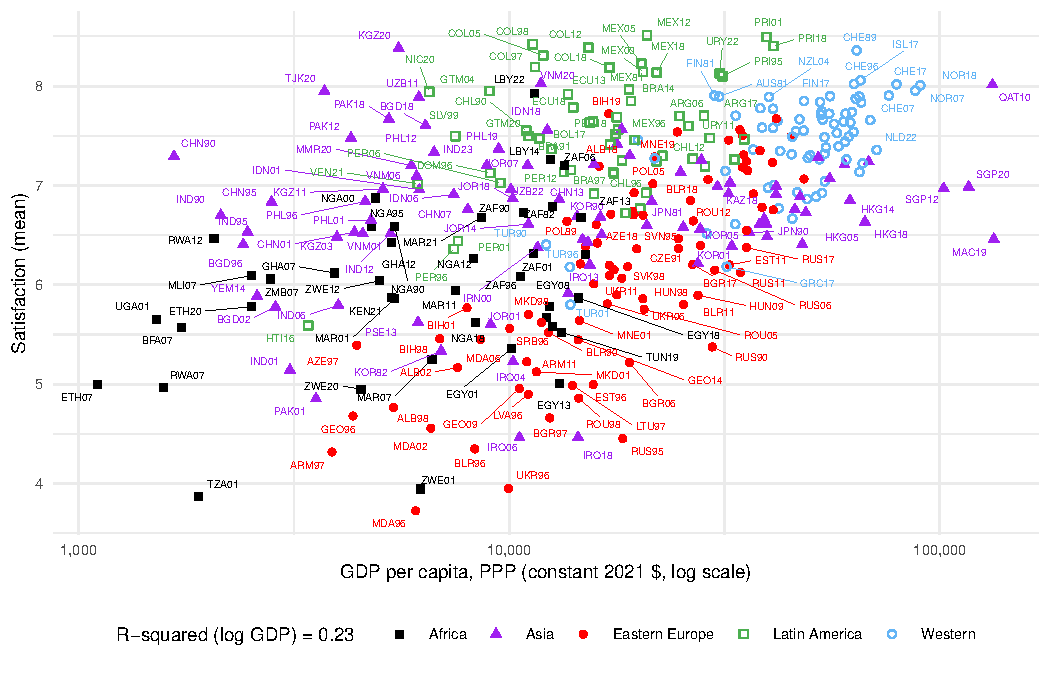
\includegraphics[width=\textwidth]{../figures/main/wvs_satisfied_mean_vs_gdp_ppp.pdf}\end{minipage}\hfill
    \begin{minipage}{.49\textwidth}\small\textit{B}\\ 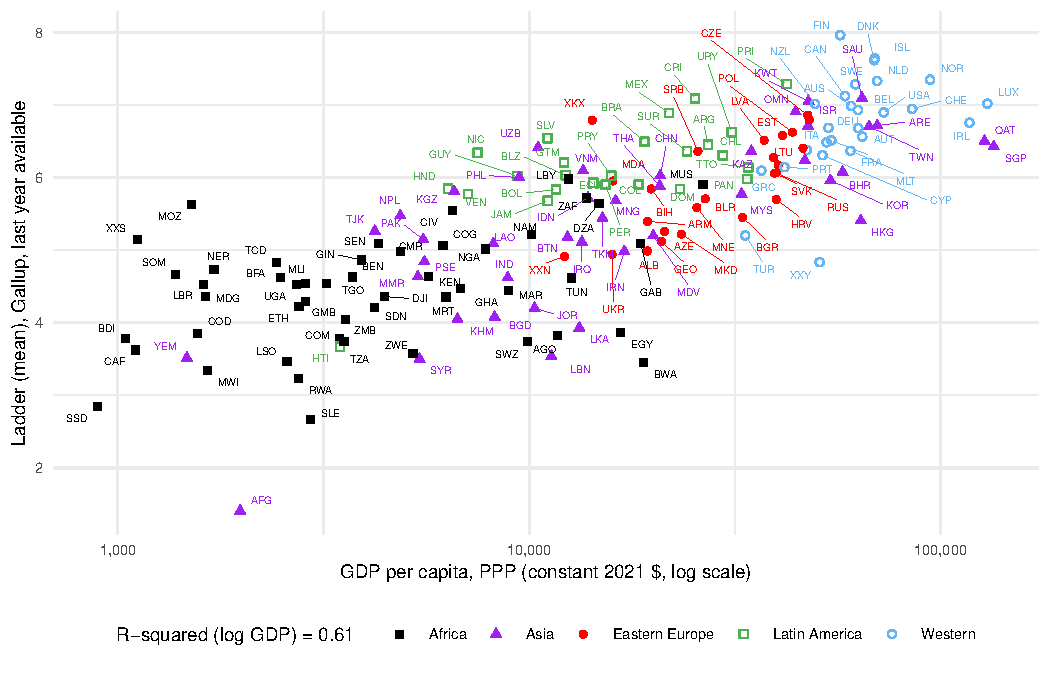
\includegraphics[width=\textwidth]{../figures/main/gallup_ladder_mean_vs_gdp_ppp.pdf}\end{minipage}\\[1ex]
    \begin{minipage}{.49\textwidth}\small\textit{C}\\ 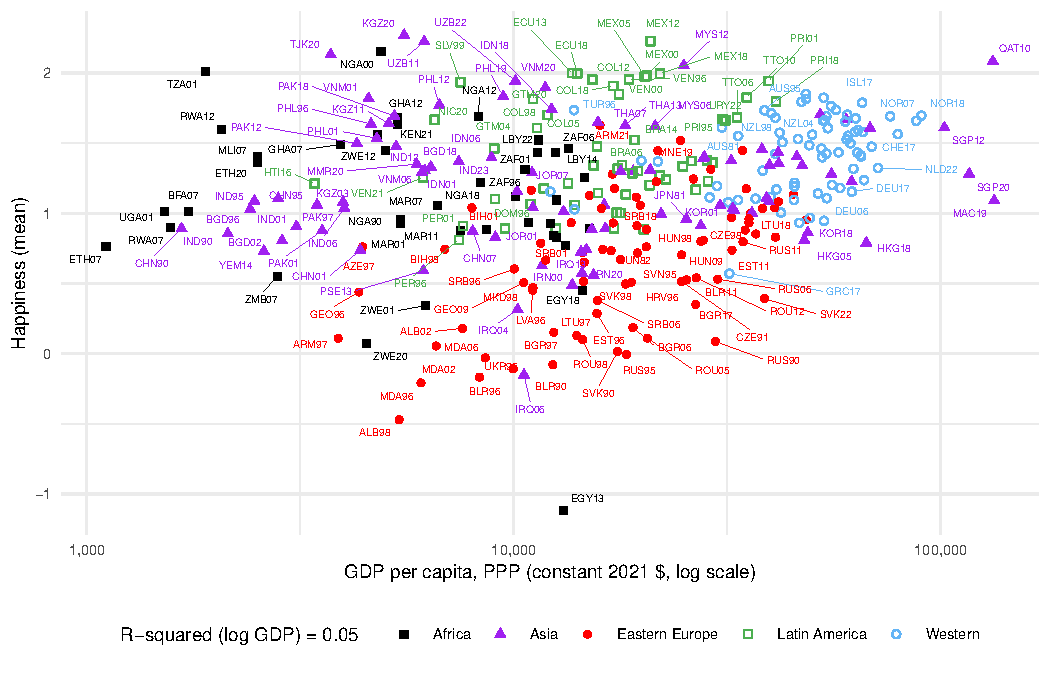
\includegraphics[width=\textwidth]{../figures/main/wvs_happiness_mean_vs_gdp_ppp.pdf}\end{minipage}\hfill
    \begin{minipage}{.49\textwidth}\small\textit{D}\\ 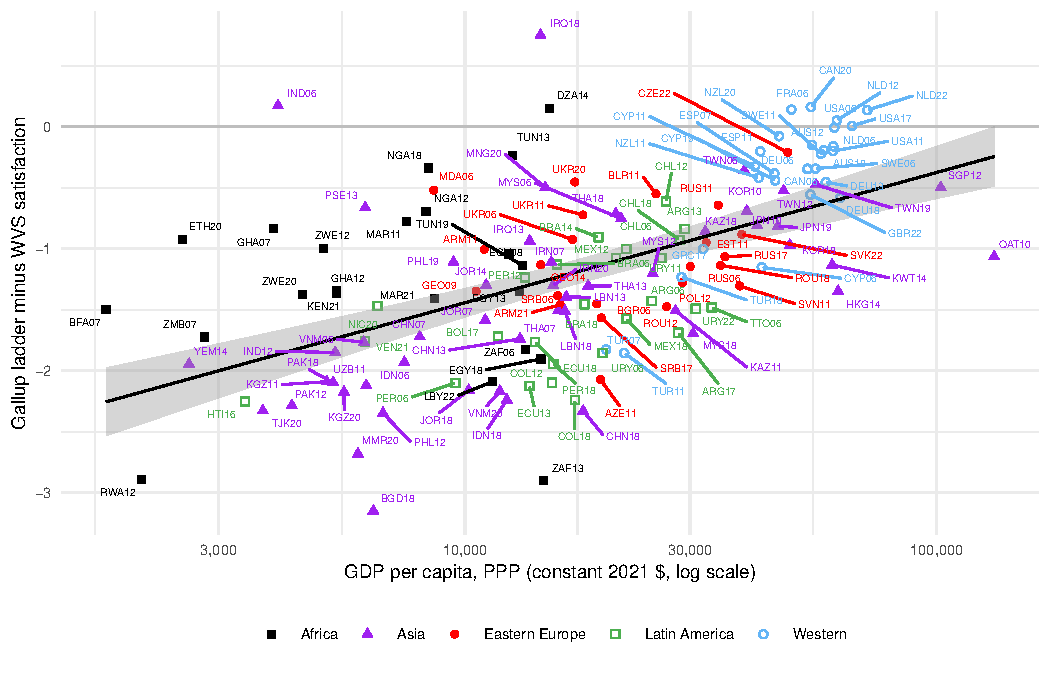
\includegraphics[width=\textwidth]{../figures/main/gap_gallup_wvs_vs_gdp.pdf}\end{minipage}
    \caption{National well-being and GDP per capita (PPP, log scale). (\textit{A}) Mean life satisfaction (1--10), WVS/EVS, \nWVSCountryYears country-years, 1981--2023 (labels: country code and year). (\textit{B}) Mean Cantril ladder (0--10), Gallup World Poll, latest observation for each of \nGallupCountries countries (2006--2023). (\textit{C}) Mean happiness, WVS/EVS (answers coded $+3$, $+1$, $-1$, $-3$ from \textit{Very happy} to \textit{Not at all happy}). (\textit{A}--\textit{C}) Colors and shapes: world regions; legends give the $R^2$ of the regression on log GDP per capita. (\textit{D}) Mean WVS life satisfaction minus mean Gallup ladder in the same country-year, \nCommon country-years observed by both surveys; line: OLS fit with 95\% confidence band.}\label{fig:scatter}
\end{figure*}

\subsection*{The discrepancy is largest in low-income countries}

The discrepancy is not due to different country coverage. In the \nCommon country-years observed by both surveys, log GDP explains \RtwoCommonGallup of the variance of Gallup's mean ladder but \RtwoCommonWVS of WVS mean satisfaction, and income accounts for \shareIncomeCommonGallup\% of the variance explained jointly with region in Gallup against \shareIncomeCommonWVS\% in the WVS. WVS answers exceed Gallup answers by around two points in low-income countries, but by less than half a point in high-income countries (Fig.~\ref{fig:scatter}D; slope \slopeGapGDP per unit of $\log_{10}$ GDP, s.e.\ \seSlopeGapGDP).


\subsection*{A survey experiment separates question and sample}

Gallup asks the Cantril ladder on a 0--10 scale; the WVS asks life satisfaction on a 1--10 scale. The surveys also differ in sampling frames, interview modes (telephone or face-to-face for Gallup; mostly face-to-face for the WVS), questionnaire context %, translations 
and survey years, which I refer to as ``samples'' in a broad sense. In an online survey of \nFabre respondents in ten high-income countries \citep{fabre_public_2025}, I randomly assigned each respondent to one of four versions of the question: Gallup's ladder or the WVS satisfaction question, on a 0--10 or 1--10 scale (\textit{Materials and Methods}). For each variant, I compute the mean answer in each country and regress it on log GDP per capita across the ten countries, as for Gallup and WVS country means in the same countries (Table~\ref{tab:ten} and Fig.~\ref{fig:fabre}).

The ten countries reproduce the global discrepancy: log GDP explains \RtwoTenGallup (95\% CI [\decompLowRGallup; \decompHighRGallup]) of the cross-country variance of Gallup's ladder but only \RtwoTenWVS ([\decompLowRWvs; \decompHighRWvs]) of WVS satisfaction. Asked to the same respondents, the questions reproduce much of this contrast: log GDP explains \RtwoTenFabreLadder ([\decompLowRFabreLadder; \decompHighRFabreLadder]) of the variance of the ladder 0--10 but \RtwoTenFabreSatisfaction ([\decompLowRFabreSatisfaction; \decompHighRFabreSatisfaction]) of satisfaction 1--10, and \RtwoTenFabreLadderPooled vs.\ \RtwoTenFabreSatisfactionPooled when pooling both scales of each wording. The wording thus accounts for \decompShareRWordingPooledPct\% (95\% CI [\decompLowShareRWordingPooledPct\%; \decompHighShareRWordingPooledPct\%]) of the Gallup--WVS difference in $R^2$, and samples for the rest. %: the new data lie midway between the two surveys. 
Pooling all four variants, income accounts for \shareIncomeTenFabreAll of the variance explained jointly with region, between Gallup (\shareIncomeTenGallup) and the WVS (\shareIncomeTenWVS).

\begin{table}[tbp]
    \centering
    \caption{Relation between GDP per capita and national well-being in the ten countries of the experiment: past surveys vs.\ new data. OLS across the ten countries, one observation per country. Gallup and WVS/EVS: latest WVS/EVS survey (2017--2022; Saudi Arabia: 2003) and Gallup the same year. Fabre (2025): mean answer by question variant; ``both scales'' and ``all four variants'': average of the variant means, 1--10 answers being linearly stretched to 0--10. 95\% CI of $R^2$: bootstrap resampling respondents. Standard errors of slopes robust to heteroskedasticity. $R^2$ region: regression on region dummies (Western, Asia, Eastern Europe, Latin America, Africa). Share due to income: Shapley share of the $R^2$ of the regression on log GDP and region attributed to income; values above 0.5 in bold.}\label{tab:ten}
    \begin{adjustbox}{max width=\textwidth}
    \begin{tabular}{lccccc}
\toprule
Data & Slope on $\log_{10}$ GDP & s.e. & $R^2$ income & $R^2$ region & Share due to income \\
\midrule
Gallup (ladder 0--10) & 4.20 & 0.80 & 0.75 & 0.29 & 0.78 \\
WVS/EVS (satisfaction 1--10) & 1.36 & 1.44 & 0.16 & 0.34 & 0.35 \\
\midrule
Fabre 2025: ladder 0--10 & 4.35 & 1.05 & 0.76 & 0.14 & 0.91 \\
Fabre 2025: ladder 1--10 & 2.57 & 1.36 & 0.33 & 0.50 & 0.36 \\
Fabre 2025: satisfaction 0--10 & 3.21 & 2.03 & 0.23 & 0.36 & 0.35 \\
Fabre 2025: satisfaction 1--10 & 4.05 & 2.09 & 0.31 & 0.29 & 0.52 \\
\bottomrule
\end{tabular}

    \end{adjustbox}
\end{table}

Slopes tell a different story. Both questions yield an income gradient close to Gallup's (\slopeTenGallup): \slopeTenFabreLadderPooled with the ladder and \slopeTenFabreSatisfactionPooled with satisfaction, whereas the WVS gradient is three times flatter (\slopeTenWVS). The part of the Gallup--WVS difference in slopes not due to the question is \SlopeDiffinDiff (95\% CI [\SlopeDiffinDiffLow; \SlopeDiffinDiffHigh]). With a single regressor, $R^2 = \beta^2 \mathrm{var}(x)/\mathrm{var}(y)$: the satisfaction question does not flatten the gradient, but it produces larger country-specific deviations from it. Japan is the most visible case: its mean satisfaction is \gapSatisfactionJPN points below that of any other country despite its high income, whereas its mean ladder is only \gapLadderJPN points below the next lowest. These country-specific deviations are present both in the WVS and in the new survey data. %country-specific deviations are partly captured by region in the WVS. 
By contrast, the flat WVS gradient is specific to its samples. With ten countries, these statistics are imprecise and sensitive to individual countries: excluding Japan, the share of the $R^2$ difference due to wording falls to \shareRtwoWordingPooledNoJPN\%.

\begin{figure}[tbp]
    \centering
    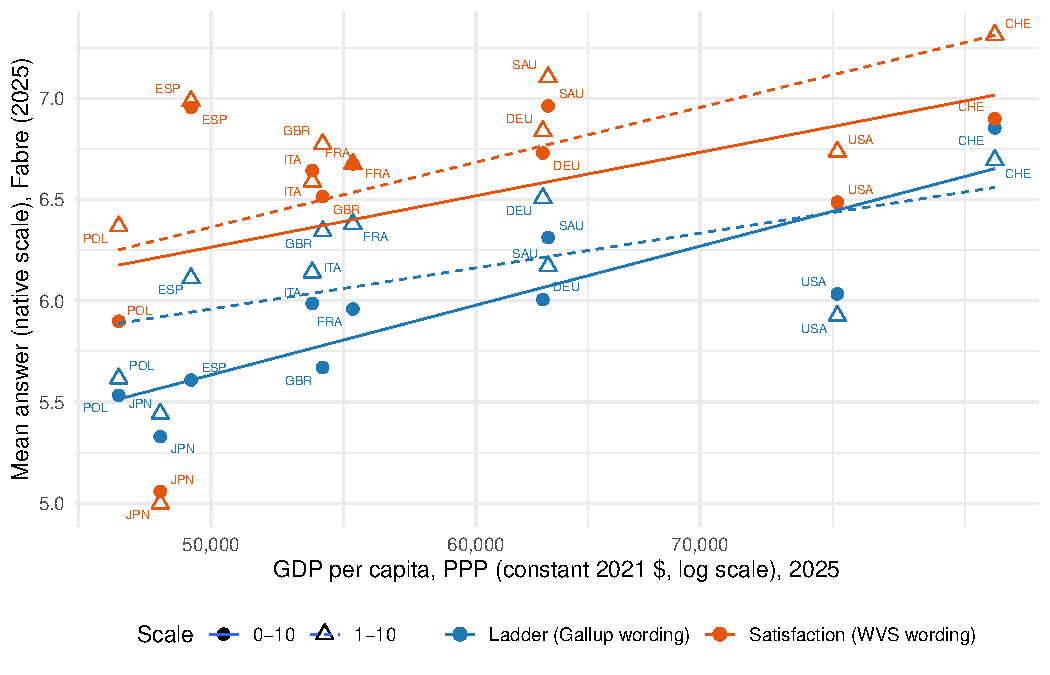
\includegraphics[width=.6\textwidth]{../figures/main/fabre_mean_vs_gdp_ppp.pdf}
    \caption{Mean life evaluation vs.\ GDP per capita (PPP, log scale) in ten countries, by randomized question variant (Fabre 2025, $n = \nFabre$). Colors: wording (Gallup's ladder or WVS life satisfaction); shapes and line types: scale (0--10 or 1--10). Mean answers on the native scale of each variant. Lines: OLS fits by variant.}\label{fig:fabre}
\end{figure}

The question also matters for levels. The ladder lowers answers by \effectLadder points on average (s.e.\ \seLadder) relative to the satisfaction question, which fully accounts for the lower level of Gallup answers in these countries: WVS answers exceed Gallup answers by \decompMeanGap points on average, and the question effect is \decompMeanQuestion points (SI Appendix, Table~S13). But the question effect does not explain why the gap varies across countries (share of the cross-country variance of the gap: \decompVarShareQuestion, 95\% CI [\decompLowVarShareQuestion; \decompHighVarShareQuestion]). Within countries, the wording does not affect the income gradient either: the interaction between the ladder wording and the respondent's income quartile is \interactionLadderIncome ($p \pInteractionLadderIncome$).

\subsection*{Neither survey is clearly more representative}

WVS samples over-represent tertiary-educated adults, by a median factor of \ratioTertiaryLow in countries with a GDP per capita below \$10,000, against \ratioTertiaryHigh above \$30,000, and over-represent urban residents in poorer countries (SI Appendix, Table~S15), as suspected by Deaton \citep{deaton_income_2008}. But correcting these imbalances has little effect: reweighting WVS samples to the population share of tertiary-educated adults changes the $R^2$ of mean satisfaction on log GDP only from \RtwoCommonWVSraw to \RtwoCommonWVSeduAdj, against \RtwoCommonGallupSub for Gallup in the same country-years. Gallup's centralized design is standardized, but it often uses only gender and age quotas, its samples are small, its microdata are not public, its modes changed during the pandemic, and part of its recent high-income interviews come from opt-in web panels \citep{gallup_methodology_2023}.

\section*{Discussion}

How much national income predicts well-being depends on the survey. In the WVS, GDP per capita explains a small share of the cross-country variance of well-being, less than a country's broad world region, because of large regional deviations: Latin America is happier, and Eastern Europe unhappier, than their income would predict. In the Gallup World Poll, income predicts as well as region. The experiment shows that both the question and the samples contribute to this discrepancy. Asked to the same respondents, the ladder is better predicted by GDP than life satisfaction, because life satisfaction produces larger country-specific deviations from the income gradient. Differences in wording reproduce about half of the difference in predictive capacity between the two surveys, the rest is attributable to the samples. %But the flat income gradient of the WVS is specific to its samples.

These results have implications for research. Cross-country conclusions about the income--well-being relationship, including rankings of the happiest countries, should be checked across surveys and questions, and the available evidence does not establish that either survey is more representative. The discrepancy is largest in low-income countries, which the experiment does not cover; replicating it face-to-face in low- and middle-income countries is the natural next step. The residual difference between surveys also lumps together sampling frames, modes, context and time, all of which can affect answers \citep{conti_survey_2011}, and which future designs could separate.

They also have implications for policy. Rich countries rarely have low life satisfaction, but middle-income countries can be as happy as the richest: the country-year with the highest mean happiness in the WVS is Kyrgyzstan in 2020, with a GDP per capita of about \$\gdpKGZ, and high life satisfaction is also reported in small-scale societies with very low monetary incomes \citep{galbraith_high_2024}. This echoes within-country evidence that income matters less for well-being than other life circumstances \citep{helliwell_hows_2003,blanchflower_well-being_2004,kahneman_would_2006}, although emotional well-being keeps rising with income for most people \citep{killingsworth_income_2023}. % and well-being rises with GDP within countries over time (SI Appendix, Table~S9). 
Growth thus does not appear necessary for high national well-being, which should be targeted directly \citep{stiglitz_report_2009,frijters_happy_2020}. Understanding the non-material factors behind regional differences---social ties, perceived freedom, culture, or response styles \citep{exton_comparing_2015,senik_french_2014}---is a priority.

\section*{Materials and Methods}

\paragraph{Well-being data.} I use the WVS time-series file \citep{wvs_trend_2022} (waves 1--7, 1981--2022), completed with the Joint EVS/WVS 2017--2022 dataset \citep{evs_wvs_joint_2024}, which adds the 2017 wave of the European Values Study and recent WVS surveys (\nWVSRespondents respondents, survey weights). As national averages of ordinal answers can be sensitive to how they are computed \citep{bond_sad_2019,kaiser_scientific_2022}, I compute eight national indicators from the happiness (4-point) and life-satisfaction (1--10) questions: the shares of happy, very happy and very unhappy people, their difference, mean happiness, mean satisfaction, the share satisfied (6--10), and the average of the shares happy and satisfied \citep{inglehart_genes_2000}. For Gallup, I use the distribution of ladder answers by country and year, tabulated from the World Poll microdata (\nGallupCountryYears country-years, 2006--2023), from which I compute the mean and six shares, and the three-year averages of the World Happiness Report \citep{whr_2026} for 2023--2025.

\paragraph{Income and regions.} Income is measured by GDP per capita at PPP (constant 2021 dollars) or at market exchange rates \citep{worldbank_wdi_2026}, in logs, in sextiles, or in $k$-means clusters ($k = 5$--7); missing values are imputed with IMF data \citep{imf_weo_2026} and growth rates. The main region classification follows the five UN regional groups: Africa, Asia (including the Middle East and Central Asia), Eastern Europe, Latin America, and Western countries. Robustness checks use six regions (isolating the Middle East), the World Bank regions, and six continents (SI Appendix).

\paragraph{Income vs.\ region.} For each indicator and income measure, I regress well-being on income, on region dummies, and on both, across country-years. The Shapley (LMG) share of the joint $R^2$ due to income is $s = [R^2_1 + (R^2_3 - R^2_2)]/(2R^2_3)$ \citep{lindeman_introduction_1980,gromping_estimators_2007}, where $R^2_1$, $R^2_2$ and $R^2_3$ are those of the three regressions; region is the better predictor if $s < 0.5$. Cross-validated $R^2$ predict each country's observations from a model estimated on all other countries. Robustness checks use each wave, population weights, the last observation per country, no EVS surveys, no pandemic years, no imputed GDP, an older GDP vintage, adjusted $R^2$, and alternative region classifications (SI Appendix, Table~S4).

\paragraph{Survey experiment.} The survey was conducted online by Bilendi (Kantar in Saudi Arabia) from April 15 to July 3, 2025, on \nFabre respondents in the United States, Japan, Saudi Arabia, Germany, the United Kingdom, France, Italy, Spain, Poland and Switzerland, with quotas on gender, age, income, education, region and urbanicity, and weights matching population frequencies. Toward the end of the questionnaire, each respondent was randomly assigned to one of four variants: the Cantril ladder (``Please imagine a ladder, with steps numbered from 0 at the bottom to 10 at the top\ldots'') or the WVS question (``All things considered, how satisfied are you with your life as a whole these days?''), with answers from 0 or from 1 to 10. The survey was approved by the CIRED institutional review board (IRB-CIRED-2025-2) %, respondents gave informed consent, 
and %the survey 
was pre-registered at \href{https://osf.io/7mzn4}{osf.io/7mzn4}. For the ten-country comparison, Gallup and WVS data are taken from the latest WVS/EVS survey of each country and the Gallup data of the same year (or at most three years apart). Confidence intervals come from 1,000 bootstrap replications resampling respondents within country and variant (experiment), within country (WVS), and answers within country (Gallup, multinomial draws). Individual-level estimates use OLS with country fixed effects and heteroskedasticity-robust standard errors.

\paragraph{Data and code availability.} Code and new data are available at \href{https://github.com/bixiou/wellbeing_gdp_region}{github.com/bixiou/wellbeing\_gdp\_region}. WVS and EVS data are freely available from the WVS Association and GESIS; Gallup World Poll data are proprietary and available from Gallup under license.

\paragraph{Acknowledgments.} I thank Claudia Senik, % whose 2016 assignment inspired this paper, % revision
participants in the 2024 STATEC Well-being Conference for helpful comments, Armon Rezai and the Vienna University of Economics and Business (WU Wien) for access to the Gallup World Poll data, and Julieta Toffoli for research assistance. This research received funding from Agence Nationale de la Recherche (ANR-24-CE03-7110). The author used Claude Opus 5.5 to write analysis code and draft parts of the manuscript, and reviewed and edited all content.

\paragraph{Author contributions.} A.F. designed research, performed research, analyzed data, and wrote the paper. \textbf{Competing interests:} The author declares no competing interest.

\bibliography{wellbeing}

\end{document}


% ---------------- SI Appendix ----------------
\clearpage
\nolinenumbers
\setcounter{table}{0}\setcounter{figure}{0}\setcounter{section}{0}\setcounter{equation}{0}
\renewcommand{\thetable}{S\arabic{table}}
\renewcommand{\thefigure}{S\arabic{figure}}
\renewcommand{\thesection}{S\arabic{section}}
\renewcommand{\theequation}{S\arabic{equation}}
\def\maketitle{\begin{center}{\LARGE Supporting Information Appendix}\\[1ex]{\large Whether richer countries are happier depends on the survey}\end{center}\bigskip}
\renewcommand{\bibliography}[1]{} % a single reference list, at the end of the main text (it includes the references cited in the SI)
\documentclass[11pt]{article}
% SI Appendix of wellbeing_pnas.tex (PNAS: single PDF, figures and tables numbered S1, S2...). Compile from papers/ (twice, with wellbeing_pnas.tex):
%   latexmk -pdf -outdir=build wellbeing_pnas_si.tex
\usepackage[T1]{fontenc}
\usepackage[utf8]{inputenc}
\usepackage{mathpazo}
\usepackage[margin=2cm]{geometry}
\usepackage[numbers,round,sort&compress]{natbib}
\usepackage{graphicx, booktabs, adjustbox, amsmath, amssymb, xcolor, caption, makecell, threeparttable}
\captionsetup{font=small, labelfont=bf}
\usepackage[colorlinks=true, urlcolor=purple, linkcolor=blue, citecolor=violet]{hyperref}
\usepackage{xspace}
\xspaceaddexceptions{]\%}
\newcommand{\corGallupWHR}{0.993\xspace}
\newcommand{\corGallupWHRoldMapping}{0.89\xspace}
\newcommand{\nGallupCountryYears}{2351\xspace}
\newcommand{\nGallupCountries}{168\xspace}
\newcommand{\nWVSCountryYears}{304\xspace}
\newcommand{\nWVSCountries}{108\xspace}
\newcommand{\nWVSRespondents}{439531\xspace}
\newcommand{\nFabre}{11000\xspace}
\newcommand{\nFabreCountries}{10\xspace}
\newcommand{\bestIncome}{Cluster k=7 nominal\xspace}
\newcommand{\shareRegionBetterWVS}{86\xspace}
\newcommand{\shareRegionBetterWVSbest}{79\xspace}
\newcommand{\nSpecsWVS}{952\xspace}
\newcommand{\meanShareIncomeBest}{28\xspace}
\newcommand{\meanRtwoIncomeBest}{19\xspace}
\newcommand{\meanRtwoIncomePPP}{12\xspace}
\newcommand{\meanRtwoRegion}{37\xspace}
\newcommand{\RtwoSatisfiedMeanPPP}{20\xspace}
\newcommand{\RtwoHappinessMeanPPP}{4\xspace}
\newcommand{\RtwoVeryHappyPPP}{0\xspace}
\newcommand{\shareRegionBetterGallup}{35\xspace}
\newcommand{\shareIncomeGallupMean}{60\xspace}
\newcommand{\RtwoGallupMeanPPP}{61\xspace}
\newcommand{\RtwoGallupRegion}{48\xspace}
\newcommand{\RtwoWHRPPP}{63\xspace}
\newcommand{\RtwoWHRRegion}{55\xspace}
\newcommand{\shareRegionBetterNoLatamEE}{27\xspace}
\newcommand{\shareIncomeNoLatamEE}{34\xspace}
\newcommand{\shareRegionBetterContinents}{54\xspace}
\newcommand{\shareRegionBetterWB}{64\xspace}
\newcommand{\cvIncomeSatisfiedMean}{0.18\xspace}
\newcommand{\cvRegionSatisfiedMean}{0.44\xspace}
\newcommand{\cvIncomeGallupMean}{0.60\xspace}
\newcommand{\cvRegionGallupMean}{0.45\xspace}
\newcommand{\shareCvRegionBetterWVS}{100\xspace}
\newcommand{\corHappySatisfied}{0.72\xspace}
\newcommand{\corHappinessSatisfactionMean}{0.76\xspace}
\newcommand{\corVeryHappySatisfiedMean}{0.63\xspace}
\newcommand{\slopeVeryHappy}{0.005\xspace}
\newcommand{\pVeryHappy}{0.85\xspace}
\newcommand{\happiestFirst}{Switzerland\xspace}
\newcommand{\happiestFirstN}{10\xspace}
\newcommand{\happiestSecond}{Mexico\xspace}
\newcommand{\happiestSecondN}{9\xspace}
\newcommand{\happiestThird}{Kyrgyzstan\xspace}
\newcommand{\happiestThirdN}{6\xspace}
\newcommand{\happiestRegionWestern}{24\xspace}
\newcommand{\happiestRegionLatinAmerica}{19\xspace}
\newcommand{\happiestRegionAsia}{16\xspace}
\newcommand{\happiestRegionAfrica}{5\xspace}
\newcommand{\nHappiestCells}{64\xspace}
\newcommand{\treeRegionFirst}{8\xspace}
\newcommand{\withinRtwoSatisfiedMean}{0.22\xspace}
\newcommand{\withinSlopeSatisfiedMean}{1.68\xspace}
\newcommand{\crossSlopeSatisfiedMean}{1.09\xspace}
\newcommand{\withinSlopeVeryHappy}{0.18\xspace}
\newcommand{\pWithinVeryHappy}{0.004\xspace}
\newcommand{\nWithin}{272\xspace}
\newcommand{\RtwoFreedomSatisfaction}{63\xspace}
\newcommand{\shapleyFreedom}{40\xspace}
\newcommand{\shapleyFreedomRegion}{26\xspace}
\newcommand{\shapleyFreedomIncome}{9\xspace}
\newcommand{\RtwoTolerance}{21\xspace}
\newcommand{\RtwoGod}{0\xspace}
\newcommand{\RtwoGrowth}{2\xspace}
\newcommand{\nonresponseSatisfactionWVS}{1.5\xspace}
\newcommand{\nonresponseHappinessWVS}{1.7\xspace}
\newcommand{\corNonresponseGDP}{-0.08\xspace}
\newcommand{\effectLadder}{-0.45\xspace}
\newcommand{\seLadder}{0.05\xspace}
\newcommand{\effectScale}{0.14\xspace}
\newcommand{\seScale}{0.05\xspace}
\newcommand{\effectLadderZeroTen}{-0.46\xspace}
\newcommand{\effectScaleZeroTen}{-0.26\xspace}
\newcommand{\effectLadderSatisfied}{-9\xspace}
\newcommand{\interactionLadderIncome}{-0.004\xspace}
\newcommand{\pInteractionLadderIncome}{0.92\xspace}
\newcommand{\gradientIncomeSatisfaction}{0.69\xspace}
\newcommand{\pHeterogeneityWording}{0.000\xspace}
\newcommand{\chiHeterogeneityWording}{93.4\xspace}
\newcommand{\wordingCHE}{-0.34\xspace}
\newcommand{\wordingDEU}{-0.53\xspace}
\newcommand{\wordingESP}{-1.12\xspace}
\newcommand{\wordingFRA}{-0.50\xspace}
\newcommand{\wordingGBR}{-0.63\xspace}
\newcommand{\wordingITA}{-0.55\xspace}
\newcommand{\wordingJPN}{0.36\xspace}
\newcommand{\wordingPOL}{-0.55\xspace}
\newcommand{\wordingSAU}{-0.79\xspace}
\newcommand{\wordingUSA}{-0.63\xspace}
\newcommand{\wordingMin}{-1.12\xspace}
\newcommand{\wordingMax}{0.36\xspace}
\newcommand{\decompMeanGap}{-0.39\xspace}
\newcommand{\decompMeanQuestion}{-0.71\xspace}
\newcommand{\decompMeanResidual}{0.32\xspace}
\newcommand{\decompShareLevelQuestion}{1.83\xspace}
\newcommand{\decompVarShareQuestion}{-0.20\xspace}
\newcommand{\decompVarShareResidual}{1.20\xspace}
\newcommand{\decompMeanAbsGap}{0.43\xspace}
\newcommand{\decompMeanAbsResidual}{0.64\xspace}
\newcommand{\decompRmsePredictionGallup}{0.73\xspace}
\newcommand{\decompRmseNaive}{0.42\xspace}
\newcommand{\decompMeanGapSat}{-0.05\xspace}
\newcommand{\decompMeanQuestionSat}{-0.11\xspace}
\newcommand{\decompVarShareQuestionSat}{-0.11\xspace}
\newcommand{\decompSdGap}{0.44\xspace}
\newcommand{\decompSdQuestion}{0.45\xspace}
\newcommand{\decompSdResidual}{0.69\xspace}
\newcommand{\decompCorGapQuestion}{-0.20\xspace}
\newcommand{\decompLowMeanGap}{-0.44\xspace}
\newcommand{\decompHighMeanGap}{-0.34\xspace}
\newcommand{\decompLowMeanQuestion}{-0.85\xspace}
\newcommand{\decompHighMeanQuestion}{-0.56\xspace}
\newcommand{\decompLowMeanResidual}{0.17\xspace}
\newcommand{\decompHighMeanResidual}{0.46\xspace}
\newcommand{\decompLowVarShareQuestion}{-0.52\xspace}
\newcommand{\decompHighVarShareQuestion}{0.15\xspace}
\newcommand{\decompLowShareLevelQuestion}{1.42\xspace}
\newcommand{\decompHighShareLevelQuestion}{2.27\xspace}
\newcommand{\decompLowCorGapQuestion}{-0.47\xspace}
\newcommand{\decompHighCorGapQuestion}{0.14\xspace}
\newcommand{\nDecompCountries}{10\xspace}
\newcommand{\nSameYear}{7\xspace}
\newcommand{\nRecent}{4\xspace}
\newcommand{\varShareQuestionSameYear}{-0.27\xspace}
\newcommand{\varShareQuestionRecent}{-0.81\xspace}
\newcommand{\shareLevelQuestionSameYear}{1.60\xspace}
\newcommand{\shareLevelQuestionRecent}{1.19\xspace}
\newcommand{\meanSampleEffectGallup}{0.75\xspace}
\newcommand{\corFabreWHR}{0.75\xspace}
\newcommand{\minSampleEffectGallup}{0.16\xspace}
\newcommand{\maxSampleEffectGallup}{1.24\xspace}
\newcommand{\meanSampleEffectWVS}{0.54\xspace}
\newcommand{\meanFabreGallupZero}{5.93\xspace}
\newcommand{\meanFabreWVSOne}{6.64\xspace}
\newcommand{\sampleEffectUSWVS}{0.49\xspace}
\newcommand{\nCommon}{149\xspace}
\newcommand{\nCommonCountries}{83\xspace}
\newcommand{\RtwoCommonGallup}{0.49\xspace}
\newcommand{\RtwoCommonWVS}{0.11\xspace}
\newcommand{\slopeCommonGallup}{1.76\xspace}
\newcommand{\slopeCommonWVS}{0.77\xspace}
\newcommand{\slopeGapGDP}{1.07\xspace}
\newcommand{\seSlopeGapGDP}{0.16\xspace}
\newcommand{\RtwoGapGDP}{0.31\xspace}
\newcommand{\slopeQuestionGDP}{0.30\xspace}
\newcommand{\seSlopeQuestionGDP}{1.75\xspace}
\newcommand{\RtwoAdjustedWVS}{0.20\xspace}
\newcommand{\shareIncomeCommonGallup}{51\xspace}
\newcommand{\shareIncomeCommonWVS}{15\xspace}

\providecommand{\newsurvey}{Fabre (2025)\xspace}
\newcommand{\Rsq}{\ensuremath{R^2}\xspace}
% \backlink{float label}{section label}: link back to the section citing a table or figure (in the combined PDF,
% to the place of the main text citing it, if any; see wellbeing_pnas_combined.tex)
\providecommand{\backlink}[2]{\if\relax\detokenize{#2}\relax\else\hfill\hyperref[#2]{(Back to Section~\ref*{#2})}\fi}
\bibliographystyle{unsrtnat}
\renewcommand{\thetable}{S\arabic{table}}
\renewcommand{\thefigure}{S\arabic{figure}}
\renewcommand{\thesection}{S\arabic{section}}
\renewcommand{\theequation}{S\arabic{equation}}

\title{Supporting Information Appendix for\\ ``Whether richer countries are happier depends on the survey''}
\author{Adrien Fabre}
\date{}

\begin{document}
\maketitle
\tableofcontents
\clearpage

\section{Data}\label{sec:si_data}
\subsection{World Values Survey and European Values Study}\label{subsec:wvs}
The World Values Survey (WVS) is the longest-running cross-national survey of values and subjective well-being. I use the WVS time-series file \citep{wvs_trend_2022}, which pools the seven waves conducted between 1981 and 2022, and complete it with the Joint EVS/WVS 2017--2022 dataset \citep{evs_wvs_joint_2024}, which adds the \nEVSSurveys national surveys of the 2017 wave of the European Values Study (EVS, conducted in 2017--2021) and \nNewWVSSurveys recent WVS surveys (India 2023, Uzbekistan 2022). The EVS asks the same well-being questions, and the combination of the two surveys is standard practice (the so-called Integrated Values Surveys). The EVS and the WVS are distinct surveys: when both surveyed the same country the same year (\nEVSSameYearWVS cases), I keep both surveys as separate observations.
For brevity, I refer to the combined data as the WVS: \nWVSRespondents respondents in \nWVSCountryYears country-years and \nWVSCountries countries. National samples are designed to be representative of the adult population, typically with 1,000 to 3,000 respondents, and most interviews are conducted face-to-face (though some recent national surveys used web, mail or mixed modes, e.g.\ the WVS in the United States in 2017 and in Japan in 2019, or the EVS in Switzerland in 2017). All statistics use the survey weights provided by the WVS and the EVS.

The WVS contains two questions on subjective well-being:
\begin{itemize}
    \item \textit{Happiness}: ``Taking all things together, would you say you are: \textit{Very happy}; \textit{Quite happy}; \textit{Not very happy}; \textit{Not at all happy}.''
    \item \textit{Life satisfaction}: ``All things considered, how satisfied are you with your life as a whole these days?'', answered on a scale from 1 (\textit{Completely dissatisfied}) to 10 (\textit{Completely satisfied}).
\end{itemize}
Non-responses are rare (\nonresponseSatisfactionWVS\% for satisfaction and \nonresponseHappinessWVS\% for happiness on average) and uncorrelated with GDP per capita (correlation: \corNonresponseGDP); they are excluded.

\paragraph{Indicators of national well-being.}
Because there is no consensus on how to aggregate ordinal answers into a national indicator, and because the ranking of countries can depend on this choice \citep{bond_sad_2019}, I compute eight indicators for each country-year:
\begin{itemize}
    \item \textit{Happy}: share answering \textit{Quite} or \textit{Very happy};
    \item \textit{Very Happy}: share answering \textit{Very happy};
    \item \textit{Very Unhappy}: share answering \textit{Not at all happy};
    \item \textit{V.~Happy -- V.~Unhappy}: difference between the two previous shares;
    \item \textit{Happiness (mean)}: mean happiness, with answers coded $+3$, $+1$, $-1$, $-3$;
    \item \textit{Satisfaction (mean)}: mean life satisfaction;
    \item \textit{Satisfied}: share answering 6 to 10 to the life-satisfaction question;
    \item \textit{Happy + Satisfied}: average of \textit{Happy} and \textit{Satisfied}, the index used by \citet{inglehart_genes_2000}.
\end{itemize}
The indicators are positively but imperfectly correlated: across country-years, the correlation between \textit{Happy} and \textit{Satisfied} is \corHappySatisfied, and between \textit{Very Happy} and \textit{Satisfaction (mean)} it is only \corVeryHappySatisfiedMean (Table~\ref{tab:correlation}). For the life-satisfaction question, I also compute the shares answering 8--10, 9--10, 10, 1--4 and 1--2, for comparisons with Gallup. 

\subsection{Gallup World Poll}\label{subsec:gallup}
The Gallup World Poll interviews around 1,000 adults per country and year in more than 140 countries, by telephone where coverage is high (typically in high-income countries) and face-to-face elsewhere \citep{gallup_methodology_2022}. Its life-evaluation question is the Cantril ladder \citep{cantril_pattern_1965}: ``Please imagine a ladder, with steps numbered from 0 at the bottom to 10 at the top. The top of the ladder represents the best possible life for you and the bottom of the ladder represents the worst possible life for you. On which step of the ladder would you say you personally feel you stand at this time?''

I use the distribution of answers by country and wave, tabulated from the Gallup World Poll microdata (\nGallupCountryYears country-years, \nGallupCountries countries, 2006--2023), from which I compute the mean and the shares answering 6--10, 8--10, 9--10, 10, 0--4 and 0--2. These distributions are unweighted. To cover the most recent years, I also use the ladder means published in the World Happiness Report 2026 \citep{whr_2026}, which average Gallup data over three years up to 2023--2025.

\subsection{Income}\label{subsec:income}
My benchmark income measure is the log of GDP per capita at purchasing power parity (PPP, constant 2021 international dollars) from the World Development Indicators \citep{worldbank_wdi_2026}. As an alternative, I use GDP per capita at market exchange rates (constant 2015 US dollars). Missing values are filled in automatically, in three steps: (i) PPP series, which start in 1990, are extended backwards (and gaps filled) using the growth rate of real GDP per capita; (ii) for countries absent from the World Bank data (e.g. Taiwan, or Venezuela in recent years), I use the IMF World Economic Outlook \citep{imf_weo_2026}, converted into the constant dollars of the World Bank series with a U.S. price deflator (the ratio of World Bank to IMF values for the United States); (iii) remaining gaps are filled with the closest year available (Montenegro 1996). Territories without national accounts use the GDP of the closest entity (e.g. the United Kingdom for Northern Ireland). A robustness check excludes all imputed values.

\subsection{Regions}\label{subsec:regions}
My main classification groups countries into the five UN regional groups (Figure~\ref{fig:regions}): \textit{Africa}, \textit{Asia} (the Asia-Pacific group, which includes the Middle East and Central Asia), \textit{Eastern Europe} (the former Eastern Bloc, excluding Central Asia), \textit{Latin America} (including the Caribbean), and \textit{Western} countries (Western Europe, North America, Australia, New Zealand, and Turkey). Territories that are not UN members (e.g.\ Taiwan, Hong Kong, Puerto Rico, Kosovo) are assigned to the group of their neighbors. 
It departs from the UN groups for two countries only: Israel, a member of the Western group since 2000 because it was denied access to the Asia-Pacific group, is classified in Asia, and Cyprus, a member of the Asia-Pacific group, is classified with Western countries. 

For robustness, I use four alternative classifications: the exact UN regional groups (with Israel in the Western group and Cyprus in Asia); a six-region variant separating the Middle East and grouping Central Asia with Eastern Europe; the seven World Bank regions (East Asia and Pacific, Europe and Central Asia, Latin America and the Caribbean, Middle East and North Africa, North America, South Asia, Sub-Saharan Africa); and six continents (Africa, North America, Latin America and the Caribbean, Asia, Europe, Oceania). The last two isolate Latin America but group Eastern and Western Europe.

See Fig.~\ref{fig:regions}.

\section{Income vs.\ region: method and additional results}\label{subsec:method_region}
For each well-being indicator and each income indicator, I estimate three linear regressions across country-years $i$:
\begin{align}
    well\text{-}being_i &= \alpha_1 + \beta_1\, income_i + u_i \label{eq:income}\\
    well\text{-}being_i &= \alpha_2 + \gamma_2\, region_i + e_i \label{eq:region}\\
    well\text{-}being_i &= \alpha_3 + \beta_3\, income_i + \gamma_3\, region_i + \varepsilon_i \label{eq:both}
\end{align}
where $region_i$ denotes the vector of region dummies. Denoting $R^2_1$, $R^2_2$ and $R^2_3$ their coefficients of determination, the share of the variance explained by income alone is $R^2_1$. To compare income and region, I decompose $R^2_3$ between the two regressors following \citet{lindeman_introduction_1980} (LMG), i.e.\ using the Shapley value \citep{gromping_estimators_2007}. With two (groups of) regressors, the LMG contribution of income is the average of its contribution when entered first ($R^2_1$) and when entered second ($R^2_3 - R^2_2$). The \textit{share of explained variance due to income} is therefore
\begin{equation}
    s = \frac{R^2_1 + (R^2_3 - R^2_2)}{2\, R^2_3}, \label{eq:share}
\end{equation}
and region is the better predictor whenever $s < 50\%$.

One feature of this comparison could favor region: region has four degrees of freedom while log GDP has one. I address this concern in three ways. First, I use categorical income variables (sextiles and clusters) with as many or more categories as regions. Second, I compute $s$ with adjusted $R^2$, which penalizes additional regressors; with more than 300 observations, the adjustment is small and only reinforces the conclusions. Third, and more directly relevant to \textit{predictive} capacity, I compute leave-one-country-out cross-validated $R^2$: each country's observations are predicted by a model estimated on all other countries. Unlike the in-sample $R^2$, the cross-validated $R^2$ decreases when a model has superfluous parameters, and it is negative when a model predicts worse than the sample mean. Other robustness checks include testing each WVS wave separately, excluding the EVS surveys, weighting countries by their population, keeping only the last observation of each country, excluding the pandemic years 2020--2021, excluding imputed GDP values, using the previous vintage of GDP data (PPP in constant 2017 dollars), alternative region classifications, and excluding Latin America or Eastern Europe.

Table~\ref{tab:region_classifications} shows that the region advantage rests on two well-known ``anomalies'': Latin America, happier than its income would predict \citep{graham_paradox_2009,rojas_handbook_2016}, and Eastern Europe, unhappier \citep{guriev_unhappiness_2009}. Region remains the better predictor when either one is excluded (in \shareRegionBetterNoLatam\% of cases without Latin America and \shareRegionBetterNoEE\% without Eastern Europe), but not when both are (\shareRegionBetterNoLatamEE\%). Consistently, the result holds with classifications that isolate both groups (exact UN groups and six regions: \shareRegionBetterUN\%), and weakens or disappears with the World Bank regions (\shareRegionBetterWB\%) and the six continents (\shareRegionBetterContinents\%), which isolate Latin America but merge Eastern and Western Europe.

The cross-sectional relation should not be confused with the relation over time. Within countries (country fixed effects, \nWithin observations), mean satisfaction increases with log GDP per capita, with a slope of \withinSlopeSatisfiedMean per unit of $\log_{10}$ GDP, larger than the cross-sectional slope (\crossSlopeSatisfiedMean), although income growth explains only \withinRtwoSatisfiedMean of the within-country variance (Table~\ref{tab:within}). These associations are consistent with \citet{stevenson_economic_2008} and \citet{sacks_new_2012} rather than with a strict version of the Easterlin paradox \citep{easterlin_does_1974,easterlin_happiness_2010}, although they may reflect common shocks (e.g.\ transition recessions) rather than the effect of income per se. Across countries, \citet{deaton_income_2008} found that, controlling for the level of GDP per capita, growth was negatively associated with life satisfaction in the 2006 Gallup World Poll. I do not find this: controlling for log GDP per capita, one percentage point of annual growth over the previous five years is associated with \growthCoefWVS points of mean satisfaction in the WVS (s.e.\ \growthSeWVS, $p \pGrowthWVS$) and \growthCoefGallup points of mean ladder in Gallup 2006--2023 (s.e.\ \growthSeGallup, $p \pGrowthGallup$), with standard errors clustered by country.

Additional results are reported in the following tables and figures: the share of explained variance due to income for each indicator and income measure (Table~\ref{tab:share_income}; Gallup: Table~\ref{tab:share_gallup}), the slopes of each indicator on log GDP (Table~\ref{tab:slopes}), other country-level correlates (Table~\ref{tab:correlates}), the countries most often ranked happiest (Table~\ref{tab:happiest}), and scatter plots of each indicator against GDP per capita (Figs.~\ref{fig:happiness_mean_gdp} and \ref{fig:very_happy_gdp}--\ref{fig:happy_gdp_w7_weighted}).

\section{Survey experiment}\label{subsec:fabre}
Gallup and the WVS differ in many respects. Gallup asks the Cantril ladder on a 0--10 scale, the WVS life satisfaction on a 1--10 scale. Gallup relies on a centralized, standardized design, with about 1,000 respondents per country every year, interviewed by telephone in high-income countries and face-to-face elsewhere; the WVS is fielded every five years or so by national teams, mostly face-to-face, with sampling designs, modes and survey years that vary across countries. These differences fall into two categories that could explain why the two datasets disagree: the question (wording and scale) and everything else---sampling frames, interview modes, questionnaire context, translations, and survey years, which I refer to as \textit{samples} in a broad sense. To separate the two, I embedded a randomized experiment in an original survey \citep{fabre_public_2025}. The survey was conducted online between April 15 and July 3, 2025, by Bilendi (or Kantar in Saudi Arabia) on \nFabre respondents in \nFabreCountries high-income countries: the United States (3,000), Japan (2,000), Saudi Arabia (1,000), Germany (1,048), the United Kingdom (826), France (798), Italy (756), Spain (603), Poland (500) and Switzerland (469); the survey also covered Russia, where the well-being question was censored. Samples were stratified with quotas on gender, age, income, education, region and urbanicity (as well as race in the U.S. and citizenship in Saudi Arabia), and results are reweighted to match population frequencies along these dimensions (with weights trimmed between 0.25 and 4).

Toward the end of the questionnaire, after questions on global policies, each respondent was randomly assigned to one of four versions of the life-evaluation question:
\begin{itemize}
    \item \textit{Ladder 0--10} (Gallup's original): the Cantril ladder question quoted in Section~\ref{subsec:gallup}, with steps numbered from 0 (\textit{Worst possible}) to 10 (\textit{Best possible});
    \item \textit{Ladder 1--10}: same wording, with steps numbered from 1 to 10;
    \item \textit{Satisfaction 0--10}: the WVS question quoted in Section~\ref{subsec:wvs}, with answers from 0 (\textit{Completely dissatisfied}) to 10 (\textit{Completely satisfied});
    \item \textit{Satisfaction 1--10} (WVS's original): same wording, with answers from 1 to 10.
\end{itemize}
This $2 \times 2$ design identifies the effect of wording (ladder vs.\ satisfaction) and scale (0--10 vs.\ 1--10), and their interaction, holding the sample, mode, context and time constant. Within each country, each branch receives around 25\% of respondents.

Although levels matter less than correlations for our question, the experiment also explains why the WVS yields higher levels than Gallup. Table~\ref{tab:fabre_regressions} reports regressions of the answer on the randomized treatments, with country fixed effects, survey weights and heteroskedasticity-robust standard errors. The ladder wording shifts answers by \effectLadder points on average (s.e.\ \seLadder): respondents rate their lives lower on the ``best possible life'' ladder than when asked how satisfied they are, in line with evidence that the ladder evokes power and wealth more than life satisfaction does \citep{nilsson_cantril_2024}. Answers on the 1--10 scale are \effectScale points higher than on the 0--10 scale (s.e.\ \seScale). Once 1--10 answers are linearly stretched to 0--10 with $x \mapsto (x-1) \times 10/9$, which maps 1 to 0 and 10 to 10, the scale effect becomes \effectScaleZeroTen: the stretch lowers each answer $x$ by $(10-x)/9$, i.e.\ by about 0.4 points at the average answer. Wording and scale do not interact. The wording effect varies markedly across countries (Figure~\ref{fig:decomposition}; $\chi^2(9) = \chiHeterogeneityWording$, $p \pHeterogeneityWording$). Japan is the exception: it is the only country where the ladder yields \textit{higher} answers than the satisfaction question (by \wordingJPN points); elsewhere, the wording effect ranges from \wordingMin (Spain) to \wordingMaxNegative points. Finally, the ladder does not steepen the income gradient \textit{within} countries: the interaction between the ladder wording and the respondent's income quartile is \interactionLadderIncome ($p \pInteractionLadderIncome$), against a gradient of \gradientIncomeSatisfaction points per quartile.

To relate these effects to the Gallup--WVS gap, I define for each country $c$ the observed gap $D_c = W_c - G_c$, where $W_c$ is mean satisfaction in the WVS and $G_c$ the mean ladder in Gallup the same year (as in the main text), and the question effect $Q_c = F_c(\text{satisfaction 1--10}) - F_c(\text{ladder 0--10})$, the difference between the mean answers to the two original variants in the experiment, measured on the same sample. The residual $R_c = D_c - Q_c$ is the part of the gap due to samples in the broad sense. On average, WVS answers exceed Gallup answers by $D = \decompMeanGap$ points, and the question effect is even larger: $Q = \decompMeanQuestion$ points (Tables~\ref{tab:decomposition_country} and \ref{tab:decomposition_summary}). The question thus fully accounts for the higher level of WVS answers in high-income countries, and the residual is small ($R = \decompMeanResidual$, 95\% CI [\decompLowMeanResidual; \decompHighMeanResidual]). Since the two components move in opposite directions, another way to summarize the level difference is to compare the size of the two movements: the question accounts for $|\bar Q|/(|\bar Q|+|\bar R|) = \decompShareAbsQuestion$ (95\% CI [\decompLowShareAbsQuestion; \decompHighShareAbsQuestion]) of the gross difference in levels.

The question effect does not, however, explain why the gap varies across countries. Since $D_c = Q_c + R_c$, the cross-country variance of the gap splits into $\mathrm{var}(D) = \mathrm{cov}(D,Q) + \mathrm{cov}(D,R)$. The share attributable to the question, $\mathrm{cov}(D,Q)/\mathrm{var}(D)$, is only \decompVarShareQuestion (95\% CI [\decompLowVarShareQuestion; \decompHighVarShareQuestion]): countries with a larger question effect do not have a larger gap. Accordingly, predicting each country's Gallup mean by subtracting its own question effect $Q_c$ from its WVS mean does worse (root mean squared error: \decompRmsePredictionGallup) than simply subtracting the average gap (\decompRmseNaive). Samples asked the same question also differ markedly. Gallup respondents (2023--2025) rate their lives \meanSampleEffectGallup points higher on the ladder 0--10 than online respondents in 2025, and WVS respondents \meanSampleEffectWVS points higher on satisfaction 1--10 (even in the United States, where the 2017 WVS was itself conducted online: \sampleEffectUSWVS points). And in the \nEVSvsWVS countries surveyed separately by the EVS and the WVS in 2017--2022, with the same question, mean satisfaction differs by \meanAbsDiffEVSWVS points on average (up to \maxAbsDiffEVSWVS).

\section{Representativeness of the surveys}\label{subsec:data_quality}
If samples matter, which dataset is closer to the truth? There is no clear-cut argument in favor of either dataset, nor of the online sample used in the experiment. Gallup applies a centralized, standardized design: probability samples of about 1,000 adults per year, drawn by random-digit dialing where telephone coverage is high and by multistage area sampling elsewhere, with random selection of the respondent within the household and post-stratification weights on gender, age and, where possible, education \citep{gallup_methodology_2023}. But its samples are small; its face-to-face samples select households by random route, with replacement of non-responding households; response rates are not published; interviews switched from face-to-face to telephone during the pandemic; and in 2023, a fifth of the interviews in 27 high-income countries came from web panels, most of them opt-in \citep{gallup_methodology_2023}. Its subgroup estimates have also been questioned \citep{blanchflower_gallup_2024}. Besides, Gallup microdata are not public, so that the representativeness of its samples cannot be assessed independently; lacking quotas, its samples could under-represent hard-to-reach groups such as less educated or rural people. The WVS requires probability samples of at least 1,200 respondents but allows quota selection at the last stage, and its sampling designs, modes and survey years vary across countries \citep{wvs_rules_wave8}. %Tests flagging near-duplicate interviews (pairs of respondents giving identical answers to almost all questions, a possible sign of fabrication) in international survey programs \citep{kuriakose_dont_2016} have been disputed \citep{pew_data_2016}. Finally, online panels exclude people without internet access, and quotas on observable characteristics do not guarantee representativeness in unobservable ones.

I test the representativeness of WVS/EVS samples directly (Table~\ref{tab:representativeness}). Compared with population benchmarks \citep{barro_new_2013,worldbank_wdi_2026}, WVS samples over-represent tertiary-educated adults (aged 25 and over) by a median factor of \ratioTertiaryLow in countries with a GDP per capita below 10,000 dollars, against \ratioTertiaryHigh in countries above 30,000 dollars (\nCompositionSurveys surveys). They also over-represent urban residents in poorer countries (median ratio \ratioUrbanLow vs.\ \ratioUrbanHigh) and under-represent people aged 65 or more (\ratioOldLow vs.\ \ratioOldHigh). The internal criterion of \citet{kohler_surveys_2007}---women should make up half of married or cohabiting respondents---is violated at the 5\% level in \shareGenderFlag\% of surveys. WVS samples are thus less representative in poorer countries, as noted by \citet{deaton_income_2008}, which is where their gap with Gallup is largest. However, correcting these observable imbalances has little effect. Controlling for log GDP, the over-representation of the tertiary-educated does not predict the gap (coefficient \coefTertiaryGap, s.e.\ \seTertiaryGap, $p \pTertiaryGap$), and reweighting each WVS sample to the benchmark share of tertiary-educated adults barely changes its relation with income: in the country-years also covered by Gallup, the $R^2$ of mean satisfaction on log GDP goes from \RtwoCommonWVSraw to \RtwoCommonWVSeduAdj, against \RtwoCommonGallupSub for Gallup. The discrepancy thus stems from unobserved differences in who responds, how, and in which context, which the available evidence does not allow me to attribute to one dataset rather than the other.

\clearpage
\section{Supplementary tables and figures}\label{sec:si_tables}

\begin{table}[p]
    \centering
    \caption{Share of the variance of national well-being explained by income alone ($R^2$), WVS/EVS 1981--2023.}\label{tab:r2_income}
    \begin{adjustbox}{max width=\textwidth}
    \begin{tabular}{lcccccccc}
\toprule
Well-being indicator & \multicolumn{2}{c}{log GDP p.c.} & Sextile & \multicolumn{4}{c}{Income cluster} \\ & PPP & nominal & PPP & $k$=5 PPP & $k$=6 PPP & $k$=7 PPP & $k$=7 nominal & Region \\
\midrule
Happy & 0.13 & 0.18 & 0.20 & 0.19 & 0.19 & 0.20 & 0.23 & 0.36 \\
Very Happy & 0.00 & 0.00 & 0.03 & 0.02 & 0.03 & 0.04 & 0.03 & 0.35 \\
Very Unhappy & 0.06 & 0.09 & 0.12 & 0.11 & 0.13 & 0.13 & 0.14 & 0.16 \\
V. Happy -- V. Unhappy & 0.00 & 0.01 & 0.05 & 0.03 & 0.04 & 0.05 & 0.04 & 0.36 \\
Happiness (mean) & 0.04 & 0.07 & 0.10 & 0.08 & 0.09 & 0.10 & 0.10 & 0.38 \\
Satisfaction (mean) & 0.20 & 0.26 & 0.21 & 0.19 & 0.19 & 0.21 & 0.26 & 0.48 \\
Satisfied & 0.28 & 0.35 & 0.30 & 0.28 & 0.28 & 0.30 & 0.35 & 0.45 \\
Happy + Satisfied & 0.25 & 0.32 & 0.28 & 0.27 & 0.27 & 0.29 & 0.33 & 0.46 \\
\midrule
Mean & 0.12 & 0.16 & 0.16 & 0.15 & 0.15 & 0.17 & 0.19 & 0.37 \\
Max & 0.28 & 0.35 & 0.30 & 0.28 & 0.28 & 0.30 & 0.35 & 0.48 \\
\bottomrule
\end{tabular}

    \end{adjustbox}
    \begin{minipage}{\textwidth}\footnotesize \textit{Note:} $R^2$ of the regression of each well-being indicator (rows) on each income indicator (columns), over \nWVSCountryYears WVS/EVS country-years (a few with missing GDP are excluded). The last column gives the $R^2$ of the regression on region dummies. The highest $R^2$ of each row is in bold. The replication files include an Excel version of this table with the $R^2$ of all region classifications (\texttt{tables/main/r2\_income\_all\_regions.xlsx}).\end{minipage}
    {\footnotesize\backlink{tab:r2_income}{}\par}
\end{table}

\begin{table}[p]
    \centering
    \caption{Share of explained variance due to income rather than region (LMG), WVS/EVS 1981--2023.}\label{tab:share_income}
    \begin{adjustbox}{max width=\textwidth}
    \begin{tabular}{lccccccc}
\toprule
Well-being indicator & \multicolumn{2}{c}{log GDP p.c.} & Sextile & \multicolumn{4}{c}{Income cluster} \\ & PPP & nominal & PPP & $k$=5 PPP & $k$=6 PPP & $k$=7 PPP & $k$=7 nominal \\
\midrule
Happy & 0.22 & 0.29 & 0.31 & 0.30 & 0.30 & 0.32 & 0.34 \\
Very Happy & 0.00 & 0.01 & 0.07 & 0.05 & 0.08 & 0.10 & 0.07 \\
Very Unhappy & 0.22 & 0.31 & 0.41 & 0.38 & 0.43 & 0.44 & 0.45 \\
V. Happy -- V. Unhappy & 0.01 & 0.02 & 0.09 & 0.06 & 0.09 & 0.11 & 0.08 \\
Happiness (mean) & 0.07 & 0.11 & 0.15 & 0.13 & 0.15 & 0.16 & 0.15 \\
Satisfaction (mean) & 0.25 & 0.30 & 0.25 & 0.23 & 0.23 & 0.25 & 0.30 \\
Satisfied & 0.35 & 0.41 & 0.36 & 0.34 & 0.35 & 0.37 & 0.41 \\
Happy + Satisfied & 0.31 & 0.38 & 0.35 & 0.33 & 0.34 & 0.35 & 0.39 \\
\midrule
Mean & 0.18 & 0.23 & 0.25 & 0.23 & 0.25 & 0.26 & 0.28 \\
Max & 0.35 & 0.41 & 0.41 & 0.38 & 0.43 & 0.44 & 0.45 \\
\bottomrule
\end{tabular}

    \end{adjustbox}
    \begin{minipage}{\textwidth}\footnotesize \textit{Note:} Share of the $R^2$ of Equation~\eqref{eq:both} attributed to income by the LMG (Shapley) decomposition, Equation~\eqref{eq:share}. Values below 0.5 indicate that region is the better predictor. Values above 0.5 (income is the better predictor) are in bold.\end{minipage}
    {\footnotesize\backlink{tab:share_income}{subsec:method_region}\par}
\end{table}

\begin{table}[p]
    \centering
    \caption{Out-of-sample predictive capacity: leave-one-country-out cross-validated $R^2$.}\label{tab:cv}
    \begin{adjustbox}{max width=\textwidth}
    \begin{tabular}{llccccc}
\toprule
Data & Indicator & Obs. & log GDP PPP & Best income variable & Region & log GDP PPP + Region \\
\midrule
WVS, all waves & Happy & 302 & 0.11 & 0.17 & 0.31 & 0.36 \\
WVS, all waves & Very Happy & 302 & -0.03 & -0.06 & 0.29 & 0.29 \\
WVS, all waves & Very Unhappy & 302 & 0.05 & 0.09 & 0.11 & 0.12 \\
WVS, all waves & V. Happy -- V. Unhappy & 302 & -0.02 & -0.05 & 0.30 & 0.29 \\
WVS, all waves & Happiness (mean) & 302 & 0.02 & 0.03 & 0.33 & 0.33 \\
WVS, all waves & Satisfaction (mean) & 302 & 0.18 & 0.19 & 0.44 & 0.51 \\
WVS, all waves & Satisfied & 302 & 0.26 & 0.30 & 0.42 & 0.53 \\
WVS, all waves & Happy + Satisfied & 300 & 0.23 & 0.28 & 0.42 & 0.51 \\
\midrule
WVS, last obs. per country & Happy & 108 & 0.05 & 0.10 & 0.24 & 0.26 \\
WVS, last obs. per country & Very Happy & 108 & -0.01 & -0.04 & 0.25 & 0.24 \\
WVS, last obs. per country & Very Unhappy & 108 & 0.04 & 0.04 & 0.05 & 0.07 \\
WVS, last obs. per country & V. Happy -- V. Unhappy & 108 & -0.02 & -0.06 & 0.25 & 0.24 \\
WVS, last obs. per country & Happiness (mean) & 108 & -0.04 & -0.04 & 0.26 & 0.24 \\
WVS, last obs. per country & Satisfaction (mean) & 108 & 0.13 & 0.12 & 0.36 & 0.40 \\
WVS, last obs. per country & Satisfied & 108 & 0.22 & 0.23 & 0.34 & 0.42 \\
WVS, last obs. per country & Happy + Satisfied & 108 & 0.18 & 0.20 & 0.36 & 0.42 \\
\midrule
Gallup, all years (2006--23) & Satisfaction (mean) & 2344 & 0.61 & 0.66 & 0.49 & 0.68 \\
Gallup, all years (2006--23) & Satisfied & 2344 & 0.65 & 0.72 & 0.52 & 0.72 \\
Gallup, all years (2006--23) & Unsatisfied (0/1--4) & 2344 & 0.63 & 0.65 & 0.48 & 0.68 \\
\midrule
Gallup, last obs. per country & Satisfaction (mean) & 167 & 0.60 & 0.58 & 0.45 & 0.64 \\
Gallup, last obs. per country & Satisfied & 167 & 0.65 & 0.68 & 0.52 & 0.70 \\
Gallup, last obs. per country & Unsatisfied (0/1--4) & 167 & 0.65 & 0.60 & 0.48 & 0.67 \\
\midrule
WHR, 2023--25 average & Satisfaction (mean) & 147 & 0.62 & 0.60 & 0.52 & 0.69 \\
\bottomrule
\end{tabular}

    \end{adjustbox}
    \begin{minipage}{\textwidth}\footnotesize \textit{Note:} Each country's observations are predicted with a model estimated on all other countries. Cross-validated $R^2 = 1 - \sum (y - \hat y_{\text{out-of-sample}})^2 / \sum (y - \bar y)^2$; it can be negative when a model predicts worse than the overall mean. In each row, the highest cross-validated $R^2$ among log GDP PPP, the best income variable and region is in bold.\end{minipage}
    {\footnotesize\backlink{tab:cv}{}\par}
\end{table}

\begin{table}[p]
    \centering
    \caption{Robustness: income vs.\ region across specifications and datasets.}\label{tab:robustness}
    \begin{adjustbox}{max width=\textwidth}
    \begin{tabular}{lccccccccc}
\toprule
Specification & Obs. & Countries & \multicolumn{2}{c}{$R^2$ income} & $R^2$ region & \multicolumn{3}{c}{Share of explained variance due to income} & Region better \\ & & & log PPP & best & & log PPP & best & adj. $R^2$ & (share of cases) \\
\midrule
WVS, all waves & 302 & 108 & 0.12 & 0.19 & 0.37 & 0.18 & 0.28 & 0.22 & 1.00 \\
WVS, waves 1--2 (1981--91) & 26 & 21 & 0.07 & 0.43 & 0.58 & 0.09 & 0.40 & 0.10 & 1.00 \\
WVS, wave 3 (1995--99) & 55 & 55 & 0.16 & 0.33 & 0.65 & 0.14 & 0.28 & 0.18 & 1.00 \\
WVS, wave 4 (1999--2004) & 40 & 40 & 0.19 & 0.31 & 0.33 & 0.27 & 0.47 & 0.47 & 0.43 \\
WVS, wave 5 (2004--09) & 58 & 58 & 0.21 & 0.35 & 0.49 & 0.22 & 0.38 & 0.23 & 0.98 \\
WVS, wave 6 (2010--16) & 60 & 60 & 0.08 & 0.22 & 0.27 & 0.14 & 0.41 & 0.19 & 0.96 \\
WVS, wave 7 (2017--22) & 64 & 64 & 0.07 & 0.13 & 0.26 & 0.20 & 0.31 & 0.14 & 1.00 \\
WVS, wave 7 w/o 2020--21 & 45 & 45 & 0.06 & 0.22 & 0.31 & 0.14 & 0.41 & 0.14 & 0.95 \\
WVS, population-weighted & 302 & 108 & 0.10 & 0.19 & 0.23 & 0.24 & 0.44 & 0.33 & 0.84 \\
WVS, last obs. per country & 108 & 108 & 0.10 & 0.18 & 0.33 & 0.18 & 0.32 & 0.21 & 0.96 \\
WVS, no GDP imputation & 283 & 104 & 0.12 & 0.19 & 0.38 & 0.17 & 0.28 & 0.21 & 1.00 \\
WVS, GDP PPP 2017 \$ (old) & 302 & 108 & 0.13 & 0.19 & 0.37 & 0.19 & 0.28 & 0.22 & 1.00 \\
WVS, w/o Latin Am. \& E. Europe & 185 & 68 & 0.16 & 0.27 & 0.18 & 0.34 & 0.68 & 0.54 & 0.27 \\
WVS, 6 regions & 302 & 108 & 0.12 & 0.19 & 0.35 & 0.18 & 0.28 & 0.22 & 1.00 \\
WVS, World Bank regions (7) & 302 & 108 & 0.12 & 0.19 & 0.22 & 0.31 & 0.43 & 0.38 & 0.64 \\
WVS, continents (5) & 302 & 108 & 0.12 & 0.19 & 0.20 & 0.34 & 0.46 & 0.41 & 0.54 \\
WVS, UN sub-regions & 302 & 108 & 0.12 & 0.19 & 0.40 & 0.20 & 0.29 & 0.25 & 1.00 \\
\midrule
Gallup, all years (2006--23) & 2344 & 167 & 0.42 & 0.48 & 0.42 & 0.46 & 0.51 & 0.49 & 0.31 \\
Gallup, last obs. per country & 167 & 167 & 0.42 & 0.44 & 0.41 & 0.44 & 0.48 & 0.45 & 0.37 \\
Gallup, last obs., WVS countries & 105 & 105 & 0.43 & 0.46 & 0.42 & 0.46 & 0.49 & 0.47 & 0.37 \\
Gallup, last obs., 6 regions & 167 & 167 & 0.42 & 0.44 & 0.42 & 0.43 & 0.46 & 0.44 & 0.41 \\
Gallup, last obs., WB regions & 167 & 167 & 0.42 & 0.44 & 0.38 & 0.47 & 0.50 & 0.48 & 0.29 \\
WHR, 2023--25 average & 147 & 147 & 0.63 & 0.63 & 0.55 & 0.56 & 0.56 & 0.56 & 0.00 \\
\bottomrule
\end{tabular}

    \end{adjustbox}
    \begin{minipage}{\textwidth}\footnotesize \textit{Note:} Averages over well-being indicators (8 for the WVS; 7 satisfaction indicators for Gallup; mean ladder for the WHR). ``Best'' refers to the income measure with the highest average $R^2$ in the main WVS specification (\bestIncome). ``Region better'' is the share of indicator $\times$ income-measure combinations for which $s < 0.5$; values above 0.5 are in bold. Alternative region classifications and exclusions of regions: see Table~\ref{tab:region_classifications}.\end{minipage}
    {\footnotesize\backlink{tab:robustness}{}\par}
\end{table}

\begin{table}[p]
    \centering
    \caption{Income vs.\ region by region classification and without Latin America or Eastern Europe (WVS/EVS).}\label{tab:region_classifications}
    \begin{adjustbox}{max width=\textwidth}
    \begin{tabular}{lcccccc}
\toprule
Region classification & Groups & Obs. & $R^2$ income & $R^2$ region & Share due to income & Region better \\ & & & (log PPP) & & (log PPP) & (share of cases) \\
\midrule
5 UN regional groups (main) & 5 & 340 & 0.14 & 0.33 & 0.23 & \textbf{0.98} \\
Exact UN regional groups & 5 & 340 & 0.14 & 0.33 & 0.23 & \textbf{1.00} \\
6 regions (Middle East separate) & 6 & 340 & 0.14 & 0.32 & 0.22 & \textbf{1.00} \\
World Bank regions & 7 & 340 & 0.14 & 0.19 & 0.37 & \textbf{0.55} \\
Continents & 5 & 340 & 0.14 & 0.17 & 0.40 & 0.48 \\
\midrule
Main, w/o Latin America & 4 & 285 & 0.15 & 0.30 & 0.26 & \textbf{0.70} \\
Main, w/o Eastern Europe & 4 & 256 & 0.16 & 0.22 & 0.29 & \textbf{0.73} \\
Main, w/o both & 3 & 201 & 0.18 & 0.20 & 0.35 & 0.27 \\
\bottomrule
\end{tabular}

    \end{adjustbox}
    \begin{minipage}{\textwidth}\footnotesize \textit{Note:} Averages over the eight well-being indicators. $R^2$ and share of explained variance due to income (Equation~\eqref{eq:share}) with log GDP p.c. (PPP). ``Region better'': share of the indicator $\times$ income-measure combinations for which $s < 0.5$; values above 0.5 are in bold. Region classifications are described in Section~\ref{subsec:regions}.\end{minipage}
    {\footnotesize\backlink{tab:region_classifications}{subsec:method_region}\par}
\end{table}

\begin{table}[p]
    \centering
    \caption{Share of explained variance due to income rather than region (LMG), Gallup, last observation per country.}\label{tab:share_gallup}
    \begin{adjustbox}{max width=\textwidth}
    \begin{tabular}{lccccccc}
\toprule
Well-being indicator & \multicolumn{2}{c}{log GDP p.c.} & Sextile & \multicolumn{4}{c}{Income cluster} \\ & PPP & nominal & PPP & $k$=5 PPP & $k$=6 PPP & $k$=7 PPP & $k$=7 nominal \\
\midrule
Satisfied & \textbf{0.58} & \textbf{0.61} & \textbf{0.59} & \textbf{0.58} & \textbf{0.60} & \textbf{0.59} & \textbf{0.60} \\
Very satisfied (8--10) & 0.44 & \textbf{0.51} & 0.49 & 0.47 & 0.49 & \textbf{0.51} & \textbf{0.53} \\
Extremely satisfied (9--10) & 0.16 & 0.25 & 0.24 & 0.27 & 0.22 & 0.30 & 0.28 \\
Completely satisfied (10) & 0.02 & 0.02 & 0.08 & 0.09 & 0.06 & 0.08 & 0.08 \\
Unsatisfied (0/1--4) & \textbf{0.61} & \textbf{0.60} & \textbf{0.60} & \textbf{0.59} & \textbf{0.61} & \textbf{0.60} & \textbf{0.59} \\
Dissatisfied (0/1--2) & \textbf{0.66} & \textbf{0.63} & \textbf{0.67} & \textbf{0.66} & \textbf{0.67} & \textbf{0.67} & \textbf{0.65} \\
Satisfaction (mean) & \textbf{0.60} & \textbf{0.62} & \textbf{0.59} & \textbf{0.58} & \textbf{0.60} & \textbf{0.59} & \textbf{0.60} \\
\midrule
Mean & 0.44 & 0.46 & 0.47 & 0.46 & 0.47 & 0.48 & 0.48 \\
Max & 0.66 & 0.63 & 0.67 & 0.66 & 0.67 & 0.67 & 0.65 \\
\bottomrule
\end{tabular}

    \end{adjustbox}
    \begin{minipage}{\textwidth}\footnotesize \textit{Note:} \nGallupCountries countries, last Gallup observation available (2006--2023). Same definitions as Table~\ref{tab:share_income}. Values above 0.5 (income is the better predictor) are in bold.\end{minipage}
    {\footnotesize\backlink{tab:share_gallup}{subsec:method_region}\par}
\end{table}

\begin{table}[p]
    \centering
    \caption{Correlation between national well-being indicators (WVS country-years).}\label{tab:correlation}
    \begin{adjustbox}{max width=\textwidth}
    \begin{tabular}{lcccccccc}
\toprule
& Happy & Very Happy & Very Unhappy & V. Happy -- V. Unhappy & Happiness (mean) & Satisfaction (mean) & Satisfied & Happy + Satisfied \\
\midrule
Happy & 1.00 & 0.61 & -0.73 & 0.70 & 0.90 & 0.72 & 0.72 & 0.90 \\
Very Happy & 0.61 & 1.00 & -0.38 & 0.98 & 0.89 & 0.63 & 0.53 & 0.61 \\
Very Unhappy & -0.73 & -0.38 & 1.00 & -0.55 & -0.68 & -0.57 & -0.57 & -0.68 \\
V. Happy -- V. Unhappy & 0.70 & 0.98 & -0.55 & 1.00 & 0.95 & 0.69 & 0.60 & 0.69 \\
Happiness (mean) & 0.90 & 0.89 & -0.68 & 0.95 & 1.00 & 0.76 & 0.70 & 0.84 \\
Satisfaction (mean) & 0.72 & 0.63 & -0.57 & 0.69 & 0.76 & 1.00 & 0.96 & 0.93 \\
Satisfied & 0.72 & 0.53 & -0.57 & 0.60 & 0.70 & 0.96 & 1.00 & 0.95 \\
Happy + Satisfied & 0.90 & 0.61 & -0.68 & 0.69 & 0.84 & 0.93 & 0.95 & 1.00 \\
\bottomrule
\end{tabular}

    \end{adjustbox}
    \begin{minipage}{\textwidth}\footnotesize\end{minipage}
    {\footnotesize\backlink{tab:correlation}{subsec:wvs}\par}
\end{table}

\begin{table}[p]
    \centering
    \caption{Slope of national well-being indicators with respect to $\log_{10}$ GDP per capita (PPP).}\label{tab:slopes}
    \begin{adjustbox}{max width=\textwidth}
    \begin{tabular}{llccccc}
\toprule
Data & Indicator & Slope & s.e. & $p$-value & $R^2$ & Obs. \\
\midrule
WVS & Happy & 0.109 & 0.019 & 0.000 & 0.145 & 337 \\
WVS & Very Happy & 0.003 & 0.025 & 0.915 & 0.000 & 337 \\
WVS & Very Unhappy & \ensuremath{-}0.022 & 0.004 & 0.000 & 0.072 & 337 \\
WVS & V. Happy -- V. Unhappy & 0.024 & 0.026 & 0.356 & 0.004 & 337 \\
WVS & Happiness (mean) & 0.268 & 0.083 & 0.001 & 0.045 & 337 \\
WVS & Satisfaction (mean) & 1.144 & 0.142 & 0.000 & 0.234 & 337 \\
WVS & Satisfied & 0.237 & 0.024 & 0.000 & 0.317 & 337 \\
WVS & Happy + Satisfied & 0.173 & 0.019 & 0.000 & 0.276 & 335 \\
\midrule
Gallup & Satisfied & 0.372 & 0.017 & 0.000 & 0.655 & 2344 \\
Gallup & Very satisfied (8--10) & 0.218 & 0.018 & 0.000 & 0.442 & 2344 \\
Gallup & Extremely satisfied (9--10) & 0.065 & 0.009 & 0.000 & 0.178 & 2344 \\
Gallup & Completely satisfied (10) & 0.012 & 0.005 & 0.008 & 0.015 & 2344 \\
Gallup & Unsatisfied (0/1--4) & \ensuremath{-}0.304 & 0.012 & 0.000 & 0.639 & 2344 \\
Gallup & Dissatisfied (0/1--2) & \ensuremath{-}0.135 & 0.009 & 0.000 & 0.432 & 2344 \\
Gallup & Satisfaction (mean) & 1.779 & 0.083 & 0.000 & 0.611 & 2344 \\
\bottomrule
\end{tabular}

    \end{adjustbox}
    \begin{minipage}{\textwidth}\footnotesize \textit{Note:} OLS across country-years; standard errors clustered by country. Gallup: 2006--2023.\end{minipage}
    {\footnotesize\backlink{tab:slopes}{subsec:method_region}\par}
\end{table}

\begin{table}[p]
    \centering
    \caption{Within-country relation between national well-being and $\log_{10}$ GDP per capita (country fixed effects, WVS).}\label{tab:within}
    \begin{adjustbox}{max width=\textwidth}
    \begin{tabular}{lccccc}
\toprule
Indicator & Slope & s.e. & $p$-value & Within $R^2$ & Obs. \\
\midrule
Happy & 0.281 & 0.042 & 0.000 & 0.276 & 309 \\
Very Happy & 0.204 & 0.048 & 0.000 & 0.142 & 309 \\
Very Unhappy & \ensuremath{-}0.038 & 0.009 & 0.000 & 0.042 & 309 \\
V. Happy -- V. Unhappy & 0.242 & 0.054 & 0.000 & 0.156 & 309 \\
Happiness (mean) & 1.046 & 0.178 & 0.000 & 0.240 & 309 \\
Satisfaction (mean) & 2.275 & 0.412 & 0.000 & 0.340 & 309 \\
Satisfied & 0.434 & 0.075 & 0.000 & 0.343 & 309 \\
Happy + Satisfied & 0.361 & 0.057 & 0.000 & 0.386 & 307 \\
\bottomrule
\end{tabular}

    \end{adjustbox}
    \begin{minipage}{\textwidth}\footnotesize \textit{Note:} Countries surveyed at least twice. Standard errors clustered by country. On average over the eight indicators, the within-country $R^2$ is \meanWithinRtwo.\end{minipage}
    {\footnotesize\backlink{tab:within}{subsec:method_region}\par}
\end{table}

\begin{table}[p]
    \centering
    \caption{Other country-level correlates of national well-being: Shapley decomposition of $R^2$ (WVS).}\label{tab:correlates}
    \begin{adjustbox}{max width=\textwidth}
    \begin{tabular}{llcccccc}
\toprule
Indicator & Other variable & Obs. & $R^2$ other alone & \multicolumn{4}{c}{Shapley decomposition of $R^2$} \\ & & & & Income & Region & Other & Total \\
\midrule
Satisfaction (mean) & Freedom of choice & 334 & 0.63 & 0.11 & 0.21 & \textbf{0.42} & 0.74 \\
Satisfaction (mean) & Importance of God & 329 & 0.01 & 0.17 & \textbf{0.33} & 0.02 & 0.51 \\
Satisfaction (mean) & Tolerance (homosexuality) & 326 & 0.24 & 0.12 & \textbf{0.30} & 0.10 & 0.52 \\
Satisfaction (mean) & Importance of democracy & 216 & 0.08 & 0.13 & \textbf{0.32} & 0.02 & 0.47 \\
Satisfaction (mean) & GDP growth (5-year) & 334 & 0.02 & 0.16 & \textbf{0.34} & 0.02 & 0.52 \\
\midrule
Happiness (mean) & Freedom of choice & 333 & 0.39 & 0.02 & 0.22 & \textbf{0.27} & 0.51 \\
Happiness (mean) & Importance of God & 330 & 0.01 & 0.05 & \textbf{0.31} & 0.03 & 0.39 \\
Happiness (mean) & Tolerance (homosexuality) & 325 & 0.09 & 0.02 & \textbf{0.31} & 0.07 & 0.40 \\
Happiness (mean) & Importance of democracy & 216 & 0.03 & 0.02 & \textbf{0.28} & \ensuremath{-}0.03 & 0.27 \\
Happiness (mean) & GDP growth (5-year) & 334 & 0.01 & 0.03 & \textbf{0.31} & 0.00 & 0.34 \\
\bottomrule
\end{tabular}

    \end{adjustbox}
    \begin{minipage}{\textwidth}\footnotesize \textit{Note:} Country-year averages of WVS variables: perceived freedom of choice and control (1--10), importance of God in one's life (1--10), justifiability of homosexuality (1--10), importance of living in a democracy (1--10, waves 5--7), and average annual growth of real GDP per capita over the previous five years. Shapley decomposition of the $R^2$ of the regression on log GDP per capita, region dummies and the other variable. In each row, the largest contribution among income, region and the other variable is in bold.\end{minipage}
    {\footnotesize\backlink{tab:correlates}{subsec:method_region}\par}
\end{table}

\begin{table}[p]
    \centering
    \caption{Countries most often ranked happiest (WVS, 8 indicators $\times$ 8 samples: each wave and all waves combined).}\label{tab:happiest}
    \begin{tabular}{lcl}
\toprule
Country & Occurrences as happiest & Region \\
\midrule
Switzerland & 10 & Western \\
Mexico & 9 & Latin America \\
Kyrgyzstan & 6 & Asia \\
Australia & 5 & Western \\
Nigeria & 4 & Africa \\
Puerto Rico & 4 & Latin America \\
Vietnam & 4 & Asia \\
Colombia & 3 & Latin America \\
Finland & 3 & Western \\
Netherlands & 3 & Western \\
\bottomrule
\end{tabular}

    \begin{minipage}{\textwidth}\footnotesize \textit{Note:} Looking at all waves combined, the happiest country-year is: \happiestAllWaves. For \textit{Very Unhappy}, the happiest country-year is the one with the lowest share.\end{minipage}
    {\footnotesize\backlink{tab:happiest}{subsec:method_region}\par}
\end{table}

\begin{table}[p]
    \centering
    \caption{Effects of question wording and scale on life evaluation, Fabre (2025) survey experiment.}\label{tab:fabre_regressions}
    \begin{adjustbox}{max width=\textwidth}
    
\begingroup
\centering
\begin{tabular}{lcccccc}
   \tabularnewline \midrule \midrule
   Dependent Variables: & \multicolumn{2}{c}{Answer} & Answer (0--10 equiv.) & Satisfied (6+) & \multicolumn{2}{c}{Answer (0--10 equiv.)}\\
   Model:                                                                         & (1)            & (2)            & (3)            & (4)            & (5)            & (6)\\  
   \midrule
   \emph{Variables}\\
   Ladder wording (Gallup)                                                        & -0.451$^{***}$ & -0.455$^{***}$ & -0.456$^{***}$ & -0.088$^{***}$ & -0.464$^{***}$ & -0.494$^{**}$\\   
                                                                                  & (0.046)        & (0.067)        & (0.067)        & (0.013)        & (0.123)        & (0.172)\\   
   Scale 1--10                                                                    & 0.137$^{**}$   & 0.132          & -0.260$^{***}$ & -0.008         & -0.276$^{***}$ & -0.540$^{**}$\\   
                                                                                  & (0.046)        & (0.068)        & (0.072)        & (0.013)        & (0.046)        & (0.182)\\   
   Ladder wording (Gallup) $\times$ Scale 1--10                                   &                & 0.008          & -0.041         & 0.028          &                & 0.055\\   
                                                                                  &                & (0.092)        & (0.097)        & (0.019)        &                & (0.247)\\   
   Income quartile (1--4)                                                         &                &                &                &                & 0.689$^{***}$  & 0.635$^{***}$\\   
                                                                                  &                &                &                &                & (0.031)        & (0.043)\\   
   Income quartile (1--4) $\times$ Ladder wording (Gallup)                        &                &                &                &                & -0.004         & 0.009\\   
                                                                                  &                &                &                &                & (0.042)        & (0.058)\\   
   Income quartile (1--4) $\times$ Scale 1--10                                    &                &                &                &                &                & 0.106\\   
                                                                                  &                &                &                &                &                & (0.061)\\   
   Income quartile (1--4) $\times$ Ladder wording (Gallup) $\times$ Scale 1--10   &                &                &                &                &                & -0.022\\   
                                                                                  &                &                &                &                &                & (0.083)\\   
   \midrule
   \emph{Fixed-effects}\\
   Country                                                                        & Yes            & Yes            & Yes            & Yes            & Yes            & Yes\\  
   \midrule
   \emph{Fit statistics}\\
   Observations                                                                   & 11,000         & 11,000         & 11,000         & 11,000         & 11,000         & 11,000\\  
   R$^2$                                                                          & 0.05681        & 0.05681        & 0.05942        & 0.04208        & 0.15976        & 0.16024\\  
   \midrule \midrule
   \multicolumn{7}{l}{\emph{Heteroskedasticity-robust standard-errors in parentheses}}\\
   \multicolumn{7}{l}{\emph{Signif. Codes: ***: 0.001, **: 0.01, *: 0.05}}\\
\end{tabular}
\par\endgroup



    \end{adjustbox}
    \begin{minipage}{\textwidth}\footnotesize \textit{Note:} OLS with country fixed effects, survey weights (normalized within country) and heteroskedasticity-robust standard errors in parentheses. \textit{Ladder wording}: Cantril ladder (vs.\ WVS life satisfaction). \textit{Scale 1--10}: answers from 1 to 10 (vs.\ 0 to 10). In columns 3, 5 and 6, 1--10 answers are linearly stretched to 0--10. Columns 5 and 6 interact the treatments with the respondent's income quartile within their country; in column 6, the interaction between income and wording is \interactionLadderIncomeFull ($p \pInteractionLadderIncomeFull$) and the triple interaction is \tripleInteraction ($p \pTripleInteraction$). * $p<.05$, ** $p<.01$, *** $p<.001$.\end{minipage}
    {\footnotesize\backlink{tab:fabre_regressions}{subsec:fabre}\par}
\end{table}

\begin{table}[p]
    \centering
    \caption{Decomposition of the WVS--Gallup gap by country.}\label{tab:decomposition_country}
    \begin{adjustbox}{max width=\textwidth}
    \begin{tabular}{lllccccccc}
\toprule
Country & Year WVS/EVS (Gallup) & Survey: mode & Gallup & WVS/EVS & Gap $D$ & Ladder 0--10 & Satisf. 1--10 & Question effect $Q$ & Residual $R$ \\ & & & (1) & (2) & (1)$-$(2) & \multicolumn{2}{c}{Fabre (2025)} & & $D-Q$ \\
\midrule
Poland & 2017 & EVS: CAPI & 6.28 & 7.56 & \ensuremath{-}1.28 & 5.53 & 6.37 & \ensuremath{-}0.84 & \ensuremath{-}0.44 \\
Spain & 2017 & EVS: CAPI & 6.47 & 7.49 & \ensuremath{-}1.02 & 5.61 & 6.99 & \ensuremath{-}1.38 & 0.36 \\
Japan & 2019 & WVS: Mail & 5.94 & 6.76 & \ensuremath{-}0.82 & 5.33 & 5.00 & 0.33 & \ensuremath{-}1.15 \\
Italy & 2018 & EVS: CAPI & 6.69 & 7.28 & \ensuremath{-}0.59 & 5.99 & 6.59 & \ensuremath{-}0.60 & 0.01 \\
Germany & 2018 & WVS: CAPI & 7.15 & 7.74 & \ensuremath{-}0.58 & 6.01 & 6.84 & \ensuremath{-}0.83 & 0.25 \\
United Kingdom & 2022 & WVS: CAPI/Web/Mail & 6.76 & 7.32 & \ensuremath{-}0.56 & 5.67 & 6.77 & \ensuremath{-}1.10 & 0.55 \\
France & 2018 & EVS: CAPI & 6.79 & 7.26 & \ensuremath{-}0.47 & 5.96 & 6.68 & \ensuremath{-}0.72 & 0.25 \\
Switzerland & 2017 & EVS: Web/Mail/CAPI & 7.58 & 8.02 & \ensuremath{-}0.43 & 6.85 & 7.31 & \ensuremath{-}0.46 & 0.03 \\
Saudi Arabia & 2003 (2006) & WVS: Face-to-face & 7.06 & 7.28 & \ensuremath{-}0.23 & 6.31 & 7.10 & \ensuremath{-}0.79 & 0.57 \\
United States & 2017 & WVS: Web/Phone & 7.23 & 7.22 & 0.01 & 6.03 & 6.74 & \ensuremath{-}0.70 & 0.71 \\
\bottomrule
\end{tabular}

    \end{adjustbox}
    \begin{minipage}{\textwidth}\footnotesize \textit{Note:} Mean answers on native scales (Gallup and ladder: 0--10; WVS/EVS and satisfaction: 1--10); columns (3) and (4): Fabre (2025). The Gallup year is given in parentheses when it differs from the WVS year. Survey: mode: source of the WVS/EVS data and main interview mode(s) (CAPI: computer-assisted personal interviews).\end{minipage}
    {\footnotesize\backlink{tab:decomposition_country}{subsec:fabre}\par}
\end{table}

\begin{table}[p]
    \centering
    \caption{Decomposition of the WVS--Gallup gap: summary.}\label{tab:decomposition_summary}
    \begin{adjustbox}{max width=\textwidth}
    \begin{tabular}{lc}
\toprule
Statistic & Estimate [95\% bootstrap CI] \\
\midrule
Mean gap $D$ (Gallup $-$ WVS) & \ensuremath{-}0.60 [\ensuremath{-}0.64; \ensuremath{-}0.55] \\
Mean question effect $Q$ (wording + scale) & \ensuremath{-}0.71 [\ensuremath{-}0.84; \ensuremath{-}0.56] \\
Mean residual $R$ (sampling, mode, context) & 0.11 [\ensuremath{-}0.04; 0.26] \\
\midrule
Share of mean gap due to question ($\bar Q/\bar D$) & 1.19 [0.94; 1.45] \\
Share of gross level difference due to question ($|\bar Q|/(|\bar Q|+|\bar R|)$) & 0.86 [0.76; 0.99] \\
Same, country average ($\overline{|Q_c|/(|Q_c|+|R_c|)}$) & 0.69 [0.56; 0.72] \\
\midrule
Share of cross-country variance of $D$ due to $Q$ ($\mathrm{cov}(D,Q)/\mathrm{var}(D)$) & 0.11 [\ensuremath{-}0.33; 0.55] \\
Share of cross-country variance of $D$ due to $R$ & 0.89 [0.45; 1.33] \\
Mean absolute gap $|D|$ & 0.60 [0.56; 0.65] \\
Mean absolute residual $|R|$ & 0.43 [0.33; 0.60] \\
Correlation between $D$ and $Q$ & 0.09 [\ensuremath{-}0.26; 0.41] \\
\midrule
Mean gap, share satisfied (6+) & \ensuremath{-}0.07 [\ensuremath{-}0.08; \ensuremath{-}0.06] \\
Mean question effect, share satisfied (6+) & \ensuremath{-}0.11 [\ensuremath{-}0.14; \ensuremath{-}0.08] \\
Variance share due to $Q$, share satisfied & 0.04 [\ensuremath{-}0.33; 0.45] \\
\bottomrule
\end{tabular}

    \end{adjustbox}
    \begin{minipage}{\textwidth}\footnotesize \textit{Note:} \nDecompCountries countries. 95\% confidence intervals from 1,000 bootstrap replications resampling respondents within country $\times$ variant (Fabre) and within country (WVS). For Gallup, only the distribution of answers is available: in each country, the numbers of respondents giving each answer (0 to 10) are redrawn from a multinomial distribution with the observed shares and sample size, which is equivalent to resampling respondents.\end{minipage}
    {\footnotesize\backlink{tab:decomposition_summary}{subsec:fabre}\par}
\end{table}

\begin{table}[p]
    \centering
    \caption{Representativeness of WVS/EVS samples: sample shares relative to population benchmarks.}\label{tab:representativeness}
    \begin{adjustbox}{max width=\textwidth}
    \begin{tabular}{lcccccc}
\toprule
Measure & Surveys & \multicolumn{4}{c}{Median} & Correlation \\ & & All & GDP $<$ 10k & 10--30k & $>$ 30k & with log GDP \\
\midrule
Tertiary education, 25+ (ratio sample/benchmark) & 295 & 1.18 & 1.98 & 1.18 & 1.05 & \ensuremath{-}0.40 \\
Urban (ratio sample/benchmark) & 76 & 1.44 & 2.19 & 1.45 & 1.22 & \ensuremath{-}0.69 \\
Aged 65+ (ratio sample/benchmark) & 335 & 0.90 & 0.64 & 0.88 & 1.01 & 0.33 \\
Women among married respondents $-$ 0.5 & 337 & 0.01 & \ensuremath{-}0.00 & 0.01 & 0.01 & 0.19 \\
\bottomrule
\end{tabular}

    \end{adjustbox}
    \begin{minipage}{\textwidth}\footnotesize \textit{Note:} One observation per WVS or EVS survey. Ratios: weighted sample share divided by the population share, medians across surveys (a ratio above 1 indicates over-representation). Benchmarks (World Bank WDI): share of the population aged 25+ with at least short-cycle tertiary education (UNESCO), or with complete or incomplete tertiary education \citep{barro_new_2013} before 2011; urban population share (national definitions; sample: urban and peri-urban respondents, waves 4, 5 and 7 only); share aged 65+ among the population aged 15+ (sample: 65+ among respondents, usually 18+). Women among married: unweighted share of women among married or cohabiting respondents minus 0.5. Correlations with log GDP per capita (PPP) of the log ratios (or of the deviation).\end{minipage}
    {\footnotesize\backlink{tab:representativeness}{subsec:data_quality}\par}
\end{table}

\begin{figure}[p]
    \centering
    \caption{Main classification of countries into five world regions.}\label{fig:regions}
    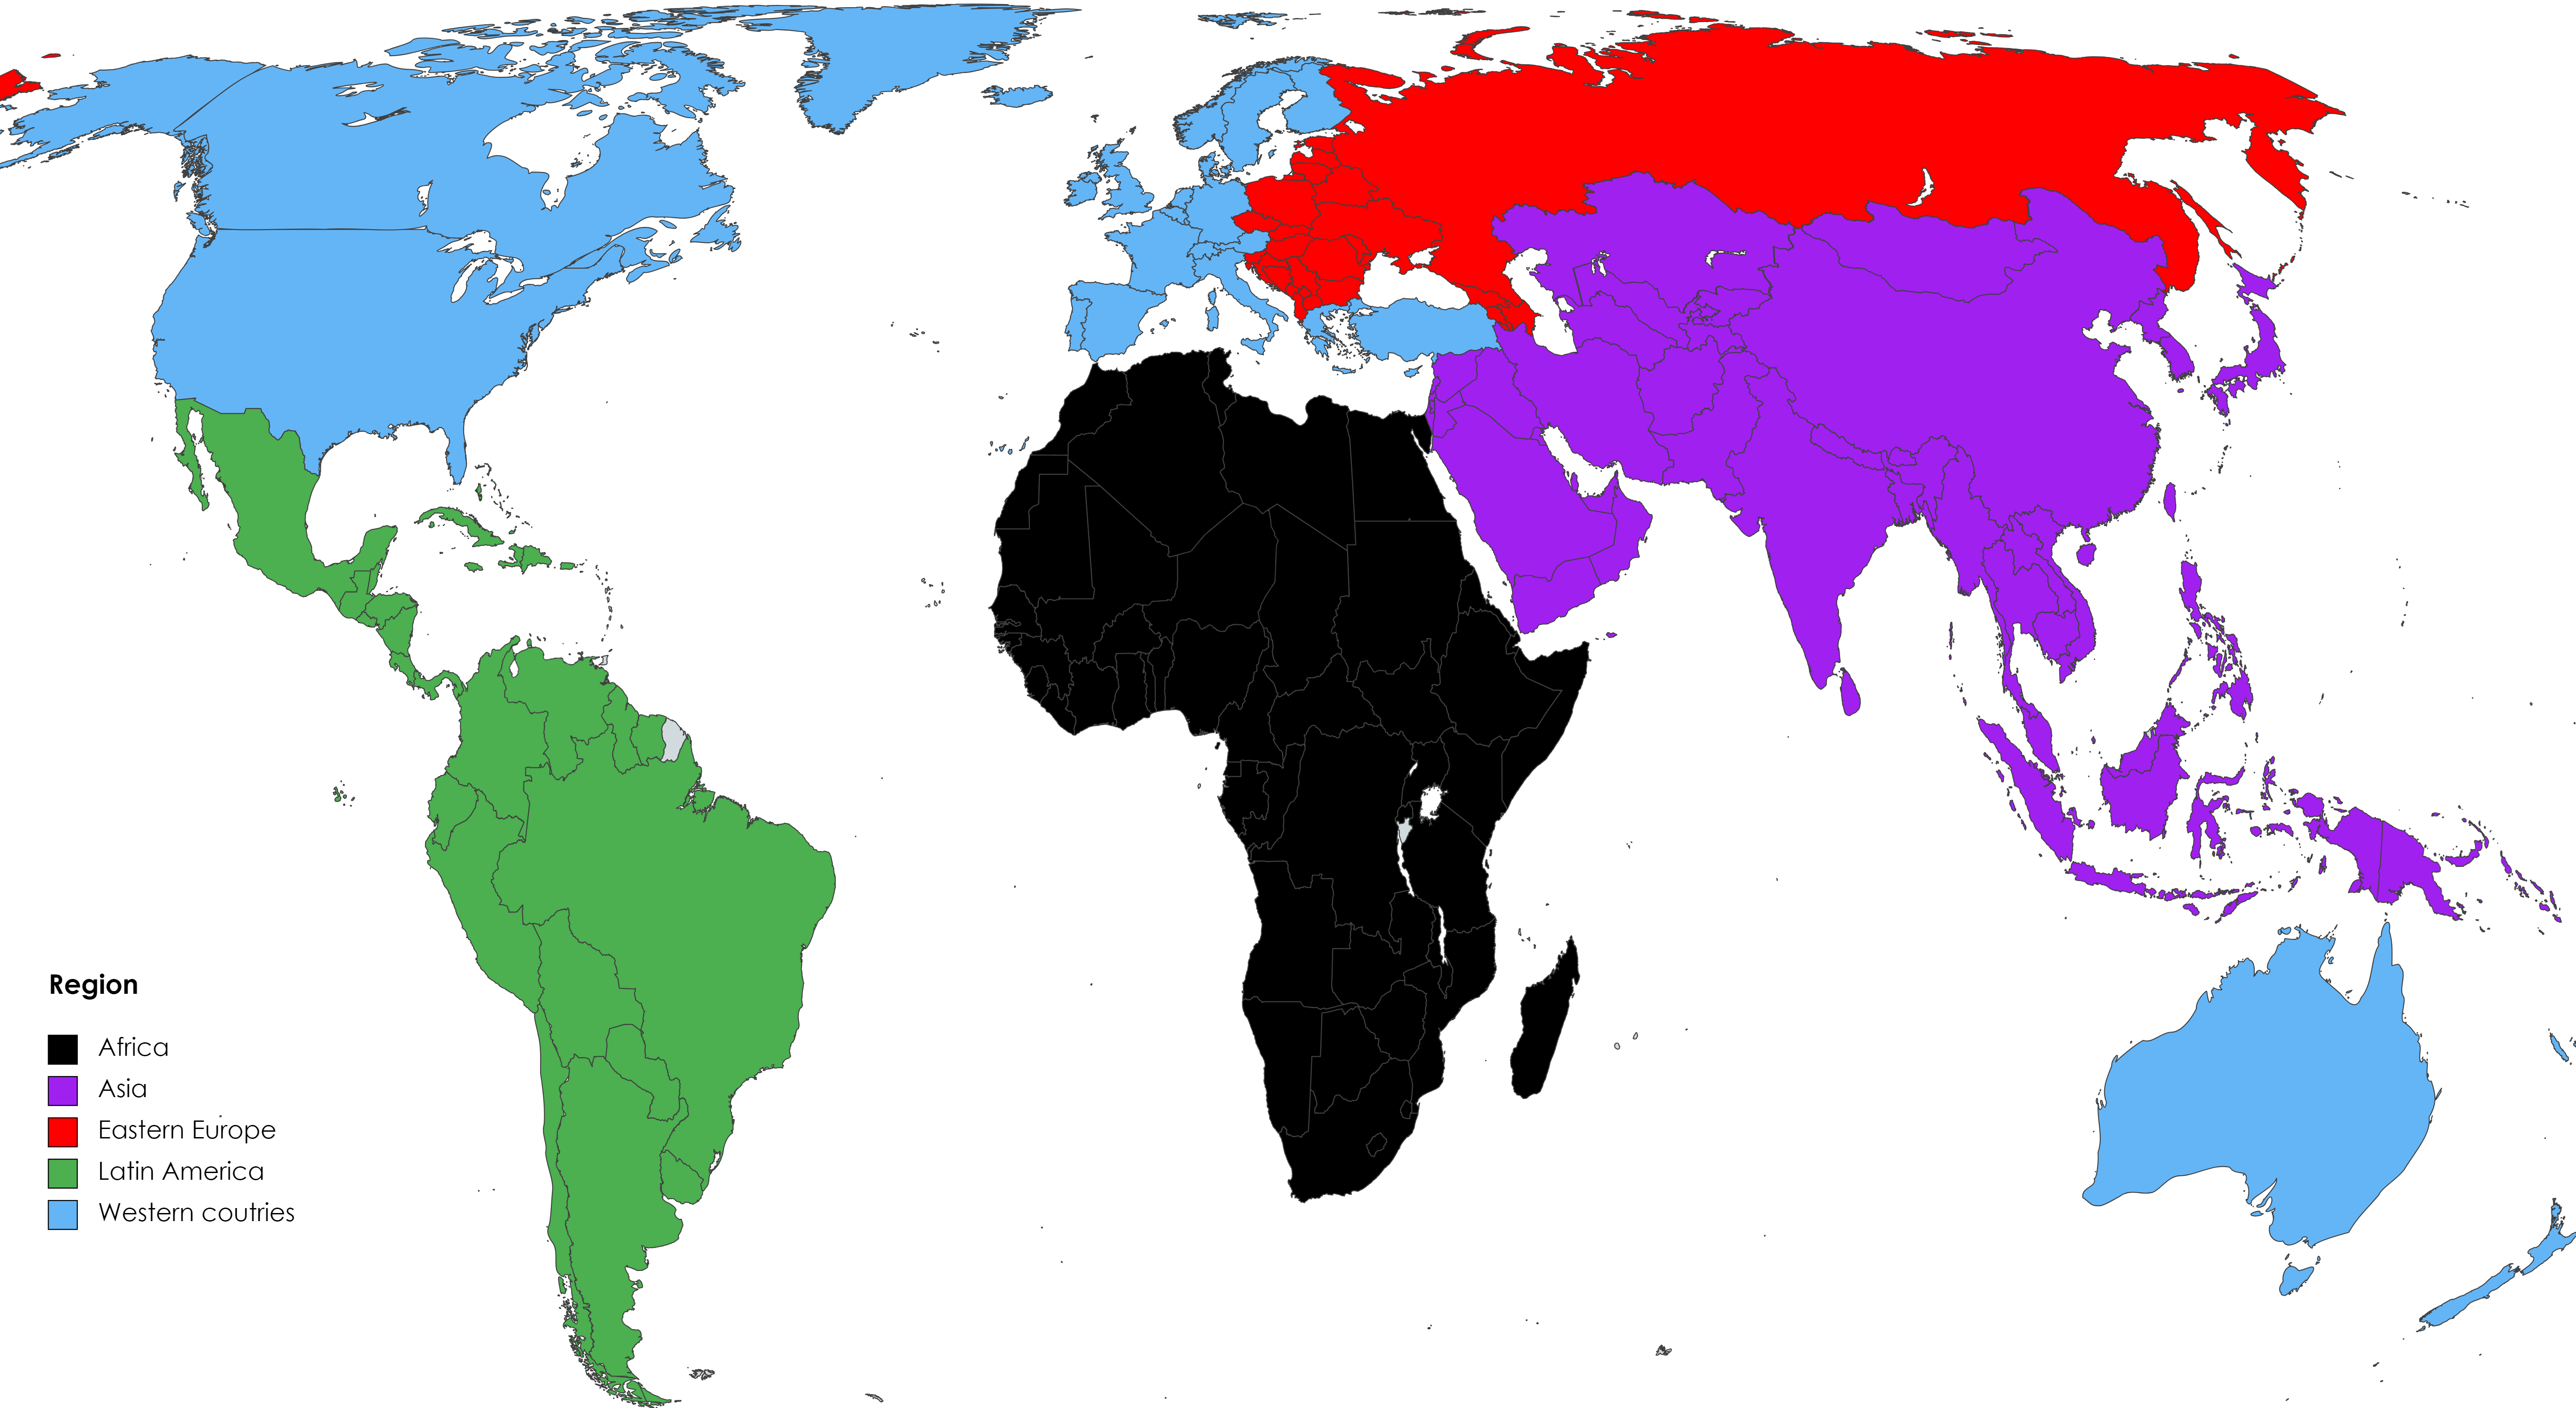
\includegraphics[width=.9\textwidth]{../figures/region_groupings.png}
    {\footnotesize\backlink{fig:regions}{subsec:regions}\par}
\end{figure}

\begin{figure}[p]
    \centering
    \caption{Mean happiness vs.\ GDP per capita (PPP), WVS/EVS 1981--2023.}\label{fig:happiness_mean_gdp}
    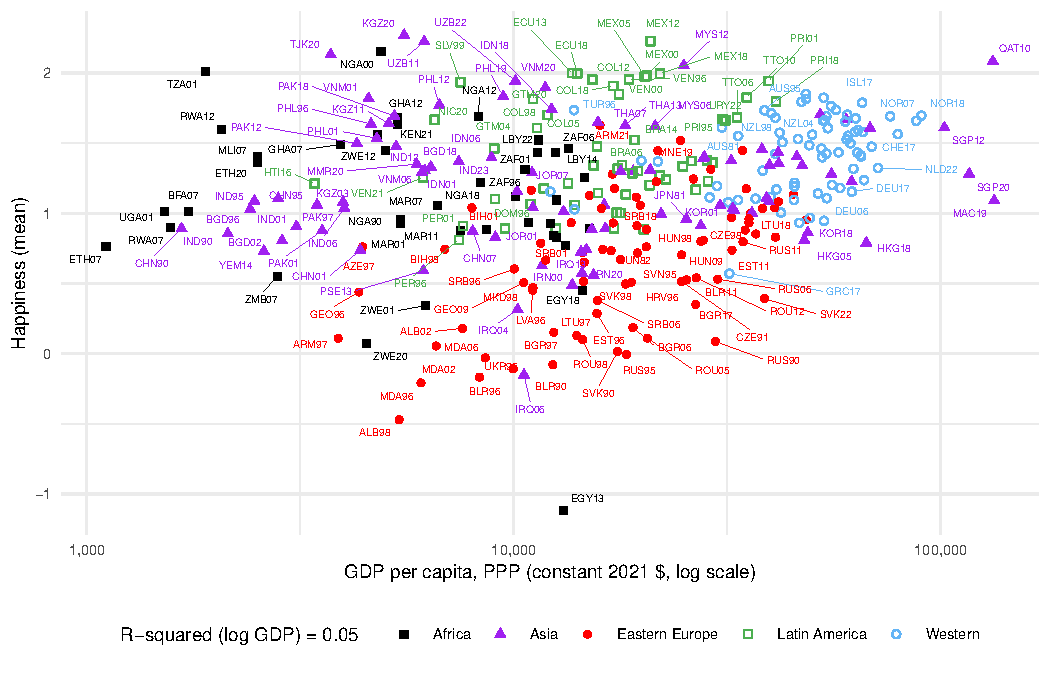
\includegraphics[width=.95\textwidth]{../figures/main/wvs_happiness_mean_vs_gdp_ppp.pdf}
    \begin{minipage}{.95\textwidth}\footnotesize \textit{Note:} Answers coded $+3$ (\textit{Very happy}), $+1$, $-1$, $-3$ (\textit{Not at all happy}).\end{minipage}
    {\footnotesize\backlink{fig:happiness_mean_gdp}{subsec:method_region}\par}
\end{figure}

\begin{figure}[p]
    \centering
    \caption{Observed WVS--Gallup gap, question effect and residual by country.}\label{fig:decomposition}
    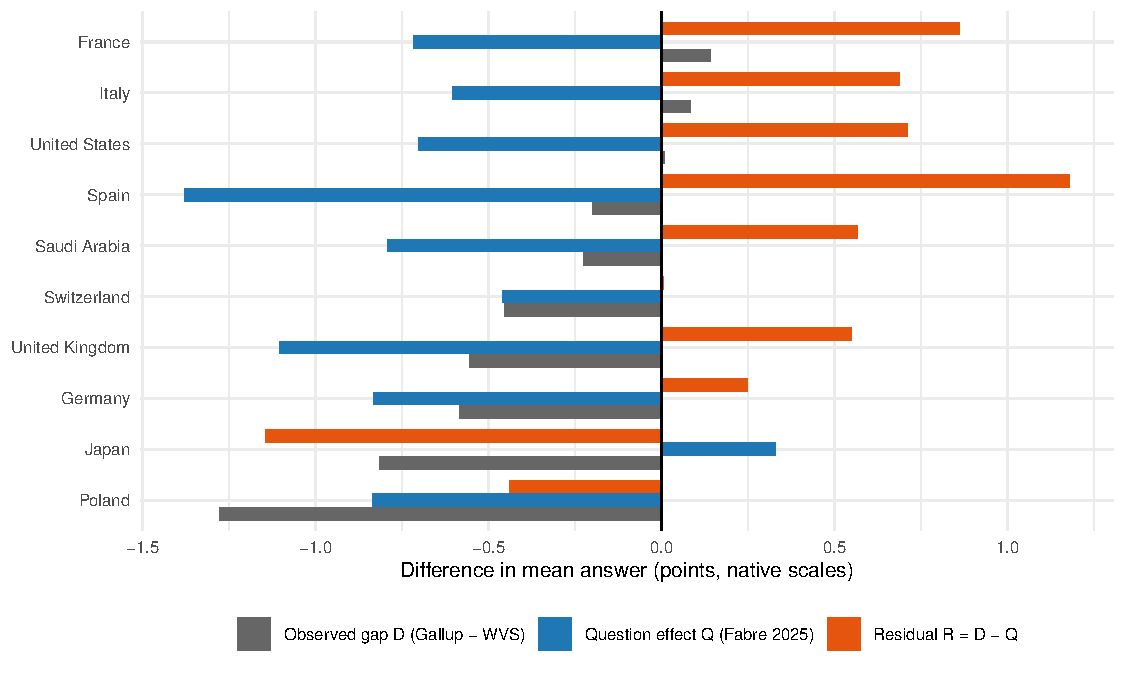
\includegraphics[width=.9\textwidth]{../figures/main/decomposition_by_country.pdf}
    \begin{minipage}{.9\textwidth}\footnotesize \textit{Note:} $D$: mean satisfaction (WVS/EVS, 1--10) minus mean ladder (Gallup, 0--10), same year. $Q$: mean answer to satisfaction 1--10 minus mean answer to ladder 0--10, Fabre (2025). $R = D - Q$.\end{minipage}
    {\footnotesize\backlink{fig:decomposition}{subsec:fabre}\par}
\end{figure}

\begin{figure}[p]
    \centering
    \caption{Share of \textit{Very happy} people vs.\ GDP per capita (PPP), WVS/EVS 1981--2023.}\label{fig:very_happy_gdp}
    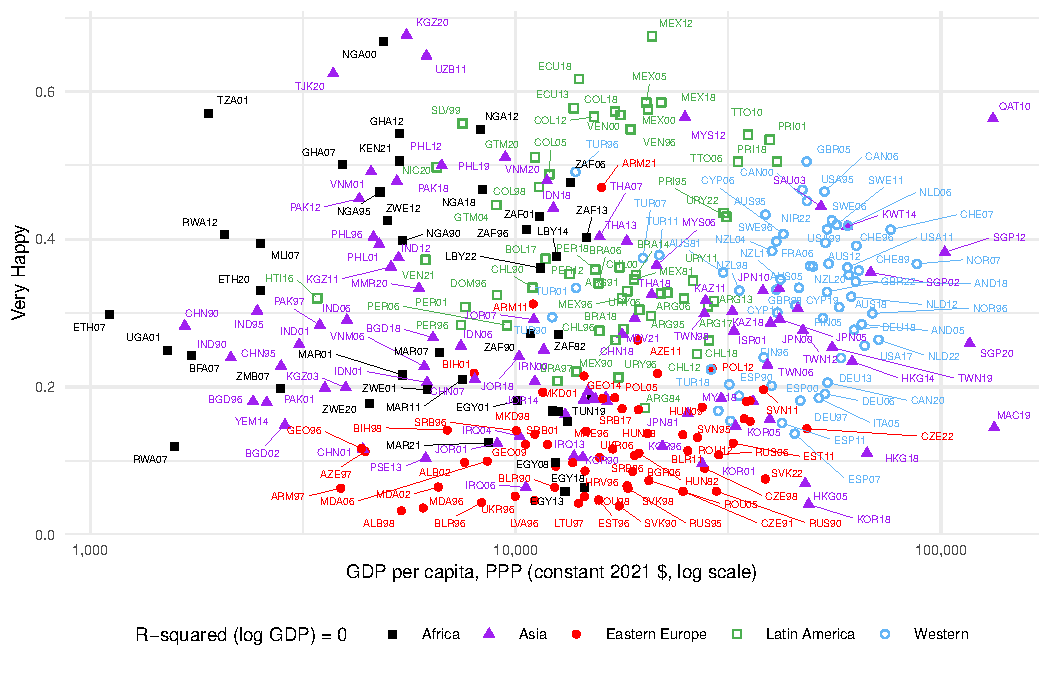
\includegraphics[width=.9\textwidth]{../figures/main/wvs_very_happy_vs_gdp_ppp.pdf}
    {\footnotesize\backlink{fig:very_happy_gdp}{subsec:method_region}\par}
\end{figure}

\begin{figure}[p]
    \centering
    \caption{\textit{Happy} vs.\ GDP per capita (PPP), WVS/EVS 1981--2023.}\label{fig:happy_gdp}
    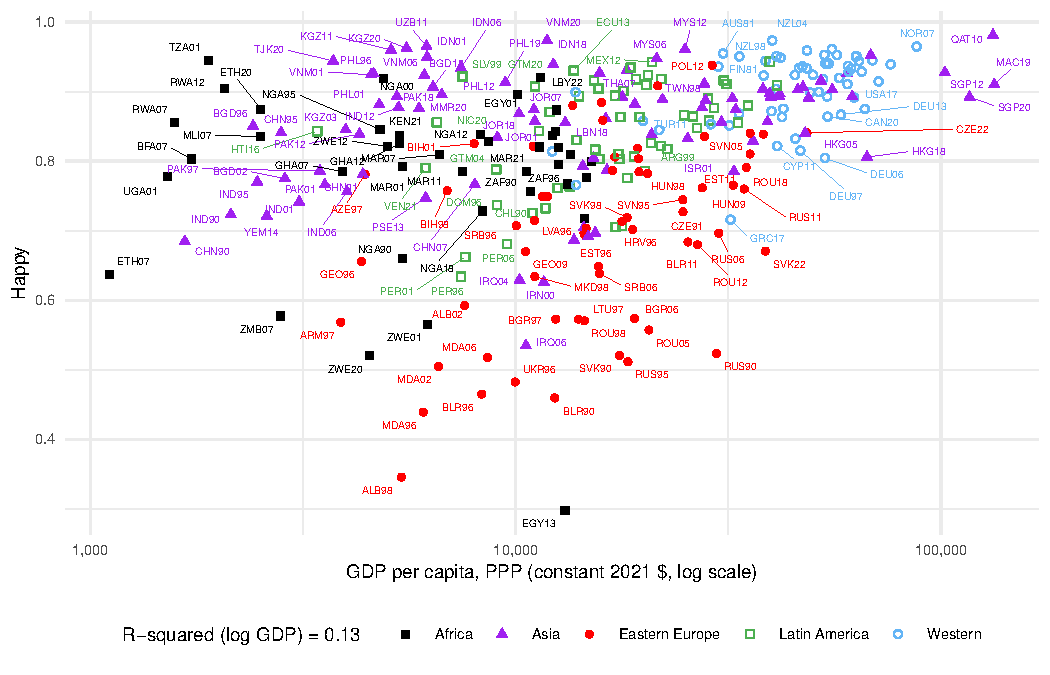
\includegraphics[width=.9\textwidth]{../figures/main/wvs_happy_vs_gdp_ppp.pdf}
    {\footnotesize\backlink{fig:happy_gdp}{subsec:method_region}\par}
\end{figure}

\begin{figure}[p]
    \centering
    \caption{\textit{Very Unhappy} vs.\ GDP per capita (PPP), WVS/EVS 1981--2023.}\label{fig:very_unhappy_gdp}
    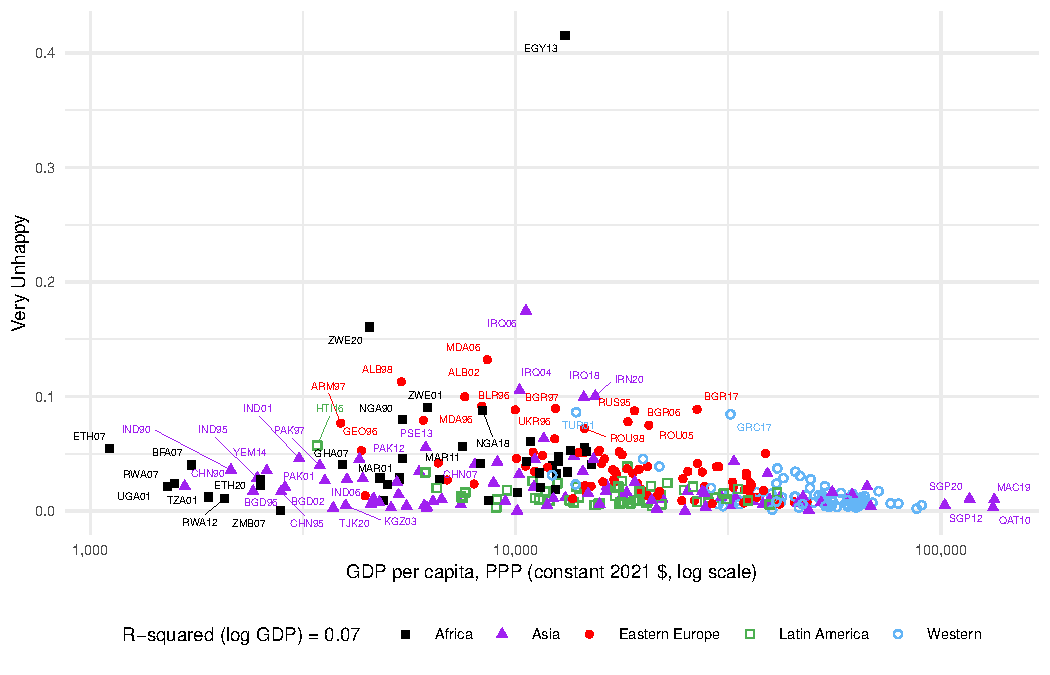
\includegraphics[width=.9\textwidth]{../figures/main/wvs_very_unhappy_vs_gdp_ppp.pdf}
    \begin{minipage}{.9\textwidth}\footnotesize \textit{Note:} Egypt 2013 (\veryUnhappyEGY\% of very unhappy people) is not shown, to keep the $y$-axis readable; the $R^2$ in the legend includes it.\end{minipage}
    {\footnotesize\backlink{fig:very_unhappy_gdp}{subsec:method_region}\par}
\end{figure}

\begin{figure}[p]
    \centering
    \caption{\textit{V.~Happy -- V.~Unhappy} vs.\ GDP per capita (PPP), WVS/EVS 1981--2023.}\label{fig:vhmvu_gdp}
    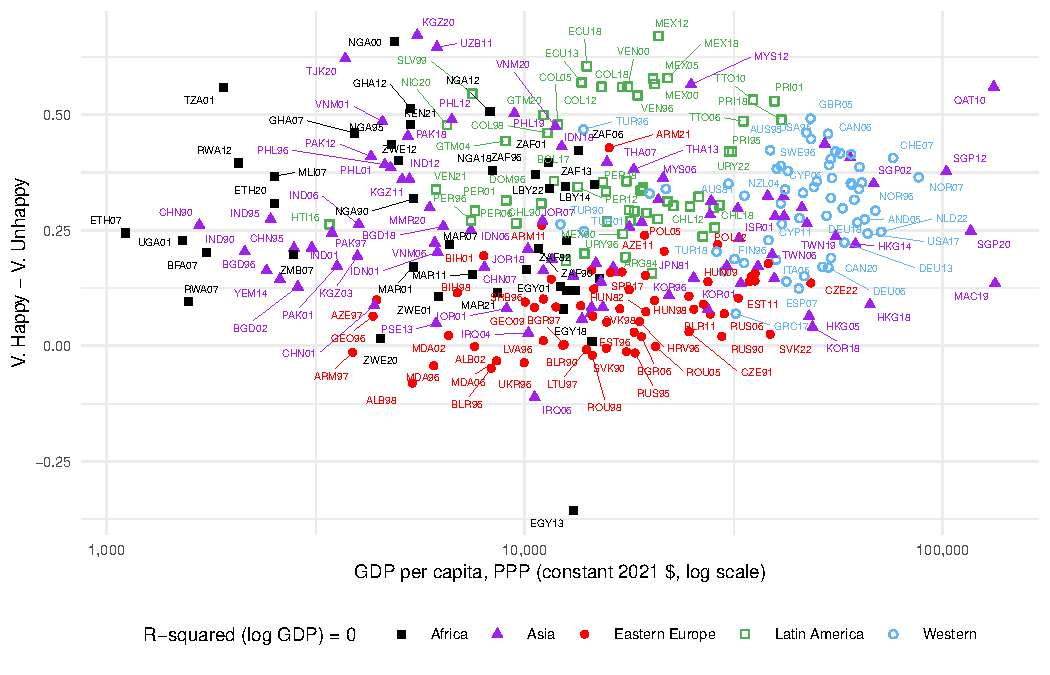
\includegraphics[width=.9\textwidth]{../figures/main/wvs_very_happy_minus_very_unhappy_vs_gdp_ppp.pdf}
    {\footnotesize\backlink{fig:vhmvu_gdp}{subsec:method_region}\par}
\end{figure}

\begin{figure}[p]
    \centering
    \caption{\textit{Satisfied} vs.\ GDP per capita (PPP), WVS/EVS 1981--2023.}\label{fig:satisfied_gdp}
    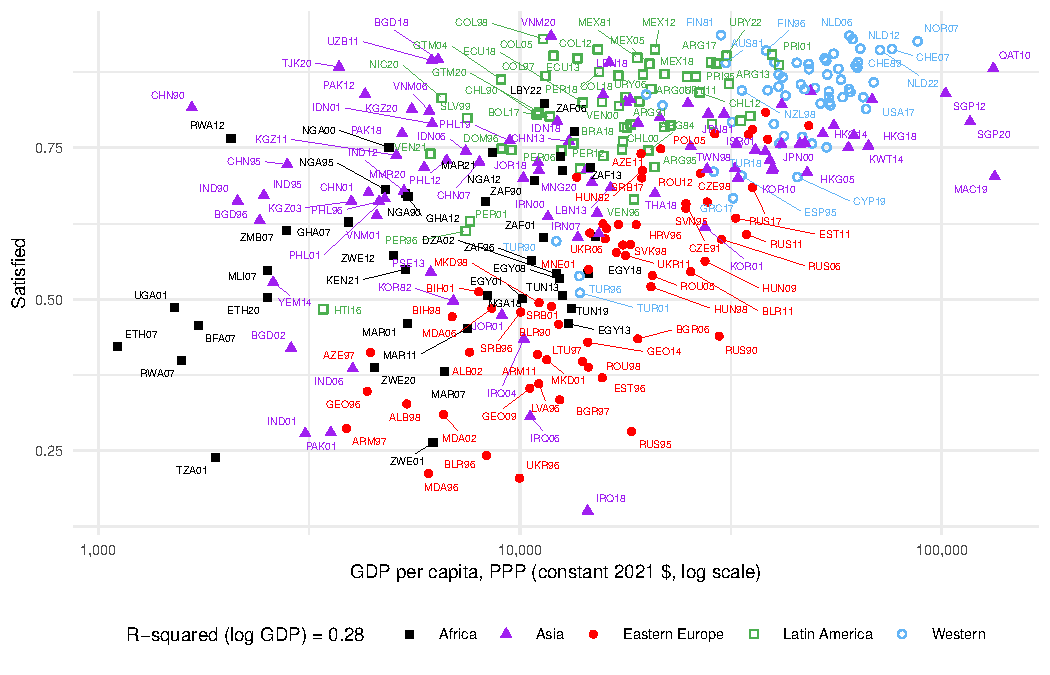
\includegraphics[width=.9\textwidth]{../figures/main/wvs_satisfied_vs_gdp_ppp.pdf}
    {\footnotesize\backlink{fig:satisfied_gdp}{subsec:method_region}\par}
\end{figure}

\begin{figure}[p]
    \centering
    \caption{\textit{Happy + Satisfied} vs.\ GDP per capita (PPP), WVS/EVS 1981--2023.}\label{fig:layard_gdp}
    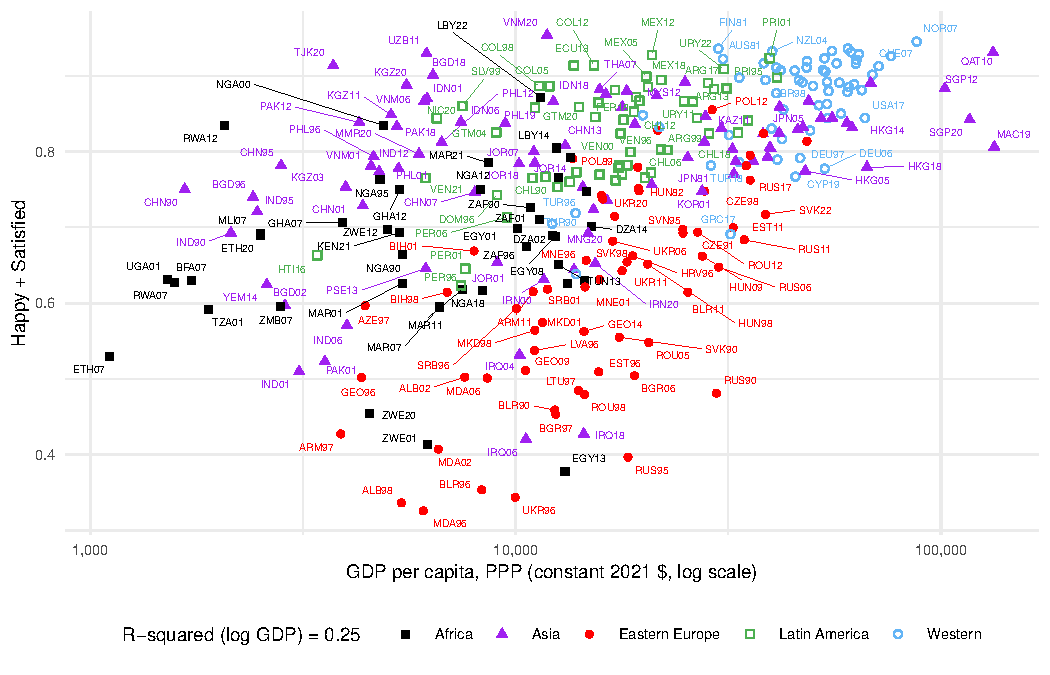
\includegraphics[width=.9\textwidth]{../figures/main/wvs_happiness_layard_vs_gdp_ppp.pdf}
    {\footnotesize\backlink{fig:layard_gdp}{subsec:method_region}\par}
\end{figure}

\begin{figure}[p]
    \centering
    \caption{\textit{Happy} vs.\ GDP per capita (nominal), WVS/EVS wave 7 (2017--2023), weighted by population.}\label{fig:happy_gdp_w7_weighted}
    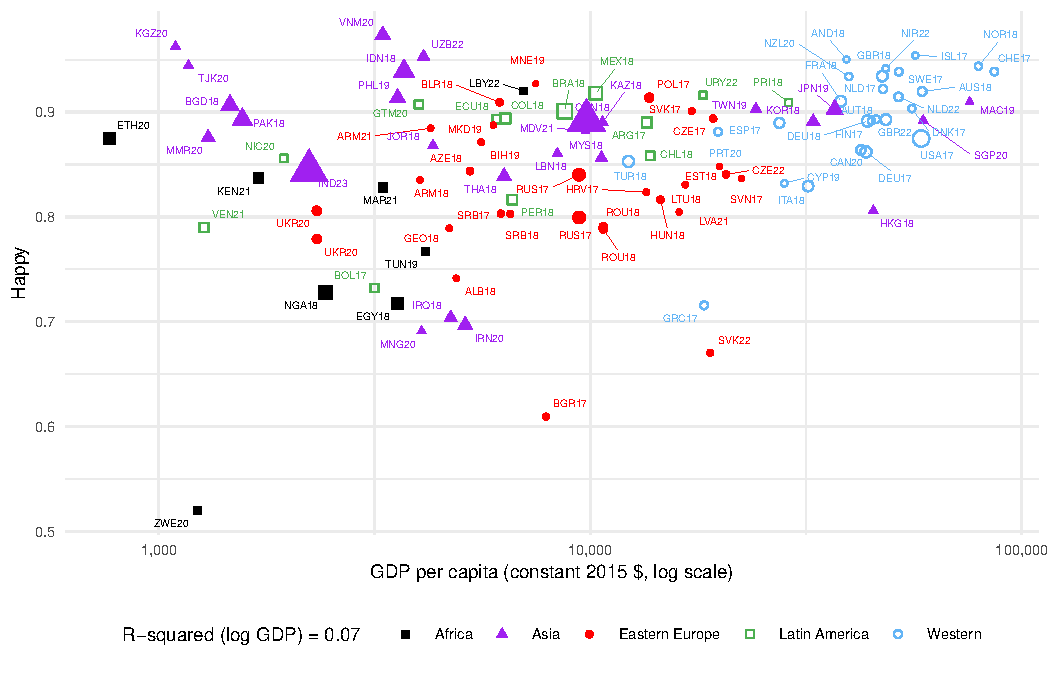
\includegraphics[width=.9\textwidth]{../figures/main/wvs_happy_vs_gdp_wave7_weighted.pdf}
    \begin{minipage}{.9\textwidth}\footnotesize \textit{Note:} Point size and regression weights proportional to population.\end{minipage}
    {\footnotesize\backlink{fig:happy_gdp_w7_weighted}{subsec:method_region}\par}
\end{figure}

\clearpage
\bibliography{wellbeing}

\end{document}

\end{document}
